\documentclass[11pt,a4paper]{report}

% =========================
% PACKAGES DE BASE
% =========================
\usepackage[utf8]{inputenc}
\usepackage[T1]{fontenc}
\usepackage[french]{babel}
\usepackage{geometry}
\usepackage{graphicx}
\usepackage{amsmath, amssymb}
\usepackage{array}
\usepackage{float}
\usepackage{hyperref}
\usepackage{tocbibind}
\usepackage{caption}
\usepackage{subcaption}
\usepackage{enumitem}
\usepackage{booktabs}
\usepackage{longtable}

% =========================
% MISE EN PAGE
% =========================
\geometry{
  left=2cm,
  right=2cm,
  top=2cm,
  bottom=2cm
}

\setlength{\parskip}{0.5em}
\setlength{\parindent}{1.5em}
\captionsetup{font=small, labelfont=bf}
\setlist[itemize]{itemsep=0.35em, topsep=0.35em}
\setlist[description]{style=nextline, font=\normalfont\bfseries, leftmargin=1.4cm}
\hypersetup{hidelinks}

% =========================
% MACROS
% =========================
\newcommand{\kw}[1]{\textbf{#1}}
\newcommand{\outil}[1]{\textbf{\texttt{#1}}}

% =========================
% INFOS DU PROJET
% =========================
\newcommand{\universite}{Université Cergy Pontoise}
\newcommand{\formation}{Master 2 IISC}
\newcommand{\ue}{Projet de synthèse}

\newcommand{\titreProjet}{Auto Fleet}

\newcommand{\auteurs}{Nom Prénom, Nom Prénom}
\newcommand{\rapporteur}{Gaussier Philippe}
\newcommand{\tuteurs}{Abdelwahed Medhi / D’Urso Raphaël}
\newcommand{\encadrant}{Tianxiao Liu}
\newcommand{\dateRendu}{08/06/2026}

% =========================
% DEBUT DOCUMENT
% =========================
\begin{document}

% =========================
% PAGE DE GARDE
% =========================
\begin{titlepage}

    \centering
    
    {\Large \universite \par}
    \vspace{0.5cm}
    {\large \formation - \ue \par}
    \vspace{2cm}
    
\includegraphics[width=0.8\textwidth]{images/logo_cy.png}

    \vspace{2cm}
    
    {\Huge \bfseries \titreProjet \par}
    \vspace{0.5cm}
    {\Large \par}
    
    \vspace{8cm}
    
    \begin{flushleft}
        \textbf{Auteurs :} Ould Younes Massyl ; Oulfid Karim ; Jianke Lin ; Kotokpo Josué \\
        \textbf{Rapporteur :} \rapporteur \\
        \textbf{Tuteurs techniques :} \tuteurs \\
        \textbf{Encadrant gestion de projet :} \encadrant \\
    \end{flushleft}
    
    \vfill
    {\dateRendu \par}
\end{titlepage}

% =========================
% REMERCIEMENTS
% =========================
\chapter*{Remerciements}
\addcontentsline{toc}{chapter}{Remerciements}

Cette section sera consolidée dans la version finale du manuscrit.

% =========================
% SOMMAIRES
% =========================
\tableofcontents
\listoffigures
\listoftables

% =========================
% INTRODUCTION
% =========================
\chapter{Introduction}

\section{Contexte du projet}

Le développement des \kw{véhicules autonomes} et des \kw{systèmes robotiques coopératifs} ne relève plus d’un simple exercice expérimental. Dans les domaines de la \kw{logistique}, de l’\kw{inspection}, de la \kw{surveillance}, de l’\kw{industrie} ou encore des \kw{environnements intelligents}, la question centrale n’est plus uniquement celle de l’autonomie d’un robot isolé, mais celle de la capacité d’un ensemble d’agents à \kw{percevoir}, \kw{décider}, \kw{se coordonner} et \kw{maintenir un service robuste} malgré les incertitudes du terrain.

L’orientation initiale du projet Auto Fleet portait sur la conception d’un robot autonome unique. Une telle approche permettait de traiter les briques fondamentales de la robotique mobile : \kw{perception locale}, \kw{odométrie}, \kw{commande}, \kw{évitement d’obstacles} et \kw{prise de décision embarquée}. Ce cadre demeurait pertinent pour poser une base méthodologique solide. Il introduisait néanmoins une limite structurelle : il n’ouvrait que partiellement la voie aux problématiques de \kw{coopération inter-agents}, de \kw{partage de données} et de \kw{supervision distribuée}.

Le projet a donc été réorienté vers une flotte de robots autonomes. Ce changement n’est pas un simple élargissement quantitatif. Il modifie la nature même du système étudié. Dès lors qu’une mission est répartie entre plusieurs unités, apparaissent des exigences nouvelles : \kw{synchronisation}, \kw{communication réseau}, \kw{cohérence des états}, \kw{cartographie partagée}, \kw{gestion des défaillances partielles} et \kw{hétérogénéité des rôles}. La difficulté ne réside plus exclusivement dans la navigation individuelle, mais dans l’intégration d’un ensemble cohérent de sous-systèmes physiques, logiciels et communicationnels.

Dans Auto Fleet, chaque robot doit ainsi maintenir une autonomie minimale de fonctionnement : acquérir des mesures, estimer son état, exécuter une commande locale, transmettre des informations utiles et rester dans un état sûr en cas de dégradation partielle de la chaîne logicielle ou réseau. À cette autonomie locale s’ajoute une logique collective : certaines données doivent être mutualisées, certains statuts partagés, et certaines représentations de l’environnement consolidées à l’échelle de la flotte.

Le projet s’inscrit en outre dans une perspective à la fois \kw{technique}, \kw{expérimentale} et \kw{pédagogique}. Les plateformes industrielles multi-robots déjà disponibles sont souvent coûteuses, peu ouvertes ou difficiles à adapter à un cadre de développement universitaire. Auto Fleet vise au contraire une base de travail \kw{modulaire}, \kw{appropriable} et \kw{évolutive}, sur laquelle peuvent être étudiés de façon concrète la \kw{locomotion omnidirectionnelle}, la \kw{fusion capteurs}, le \kw{SLAM collaboratif}, la \kw{supervision réseau} et la \kw{gestion d’une flotte hétérogène}.

\section{Un exemple d’utilisation : mise en scénario}

Un scénario représentatif du projet consiste en une mission d’exploration d’une zone forestière partiellement inconnue. L’environnement considéré n’est ni parfaitement structuré ni entièrement prédictible : il contient des obstacles naturels, des zones masquées et des passages dont l’accessibilité ne peut être présumée. Dans un tel contexte, le recours à une flotte présente un intérêt opérationnel direct : la surface explorée peut être couverte plus rapidement, les rôles peuvent être répartis, et les informations utiles peuvent être consolidées à mesure de l’avancement de la mission.

La flotte considérée dans ce scénario comprend quatre robots. Deux d’entre eux sont équipés d’un \kw{LiDAR} et participent à la construction progressive d’une carte de l’environnement selon une logique de \kw{SLAM}. Les deux autres s’appuient principalement sur une \kw{caméra} et sur leur perception locale pour progresser dans la zone, compléter l’observation du terrain et contribuer à la recherche de la cible. Cette répartition n’introduit pas une hiérarchie entre robots ; elle formalise plutôt une \kw{spécialisation fonctionnelle} destinée à réduire le coût embarqué tout en conservant une capacité collective élevée.

Pendant la mission, chaque robot exécute une navigation autonome de proximité, avec détection locale d’obstacles, adaptation de trajectoire et remontée d’état. En parallèle, des échanges réseau permettent de diffuser des informations de \kw{position}, de \kw{télémétrie}, d’\kw{événements de mission} et, pour les robots concernés, des données utiles à la \kw{cartographie partagée}. L’opérateur n’assure donc pas un pilotage point à point : il supervise un système dans lequel la décision locale demeure embarquée, tandis que la station centrale conserve une vue consolidée de la situation.

\begin{figure}[H]
    \centering
    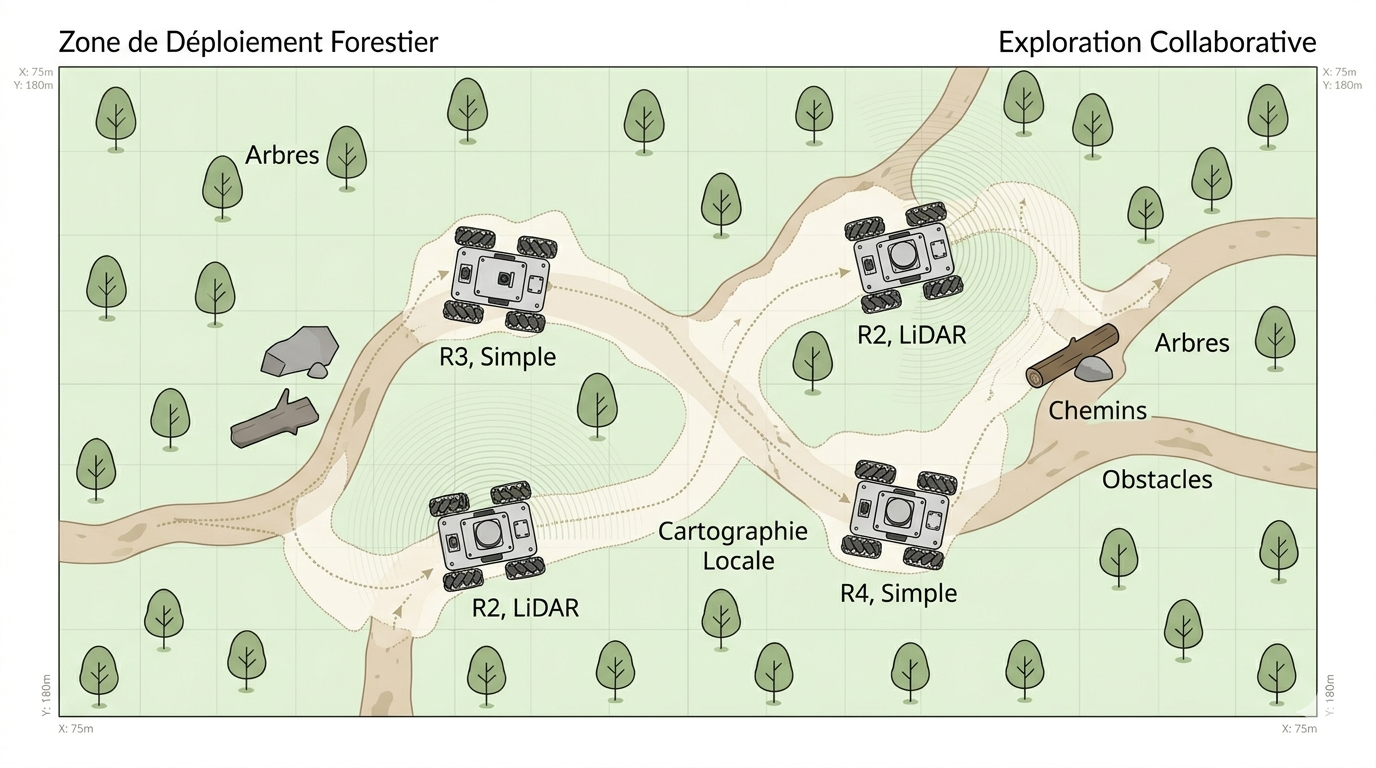
\includegraphics[width=0.95\textwidth]{images/CasUtilisation2.png}
    \caption{Scénario d’exploration collaborative en zone forestière}
    \label{fig:scenario_foret}
\end{figure}

\section{Objectifs du projet et fonctionnalités attendues}

L’objectif principal du projet Auto Fleet est la conception d’une \kw{flotte de robots autonomes collaboratifs}, depuis l’architecture embarquée jusqu’aux mécanismes de supervision. Il ne s’agit pas uniquement de faire fonctionner plusieurs robots en parallèle, mais de structurer un système capable d’assurer la \kw{cohérence fonctionnelle} d’un ensemble de sous-systèmes répartis.

Un premier objectif concerne l’\kw{architecture matérielle embarquée}. Chaque robot doit intégrer une unité de calcul, un microcontrôleur, des capteurs, des moteurs, une alimentation et des interfaces de communication dans un encombrement raisonnable. Le système ne peut être viable que si cette intégration reste \kw{maintenable}, \kw{diagnostiquable} et suffisamment \kw{modulaire} pour accepter des itérations de développement.

Un second objectif porte sur la \kw{locomotion} et la \kw{perception}. Les robots doivent être capables de se déplacer, d’asservir leurs roues, d’estimer leur mouvement et de produire une perception exploitable de leur voisinage. Cette perception repose sur plusieurs sources : \kw{LiDAR}, \kw{caméra}, \kw{IMU}, \kw{encodeurs} et, selon les cas, capteurs de proximité. L’intérêt n’est pas seulement d’accumuler des mesures, mais d’en faire une base suffisamment robuste pour soutenir la navigation et la supervision.

Le projet vise également la mise en place d’une \kw{cartographie partagée}. Les robots équipés d’un LiDAR doivent contribuer à la construction d’une représentation de l’environnement qui dépasse leur trajectoire individuelle. Cette carte n’a pas une valeur illustrative ; elle constitue une structure de référence pour la mission, pour la lecture de l’état global et, à terme, pour l’aide à la navigation des unités moins instrumentées.

Enfin, Auto Fleet intègre une dimension marquée de \kw{communication} et de \kw{supervision}. La flotte doit être observable : l’opérateur doit pouvoir identifier les robots disponibles, visualiser leur état, suivre leur progression et intervenir sans se substituer à la logique embarquée. Cette exigence conduit à structurer une chaîne complète allant du robot au backend, puis du backend à l’interface de supervision.

Les fonctionnalités attendues du système sont les suivantes :

\begin{itemize}
    \item \kw{Déplacement autonome} de robots mobiles en environnement partiellement inconnu, avec maintien d’un comportement sûr ;
    \item \kw{Commande bas niveau} des moteurs et gestion de la locomotion à quatre roues, y compris pour les plateformes à roues mécanum ;
    \item \kw{Perception locale} par combinaison de \kw{LiDAR}, \kw{caméra}, \kw{IMU}, \kw{encodeurs} et capteurs de proximité ;
    \item \kw{Détection d’obstacles} et adaptation locale de trajectoire ;
    \item \kw{Cartographie partagée} de la zone explorée par les robots instrumentés pour le \kw{SLAM} ;
    \item \kw{Communication réseau} entre robots, backend et station de supervision ;
    \item \kw{Simulation} des comportements et de l’interaction avec l’environnement ;
    \item \kw{Visualisation et contrôle} de la flotte via une \kw{IHM} dédiée.
\end{itemize}

Auto Fleet a ainsi une double portée. D’une part, il constitue un \kw{démonstrateur technique} permettant d’éprouver une architecture multi-robots cohérente. D’autre part, il fournit une base réutilisable pour des développements ultérieurs en \kw{navigation autonome}, \kw{coordination distribuée}, \kw{cartographie collaborative} et \kw{supervision d’essaims robotiques}.

\begin{figure}[H]
    \centering
    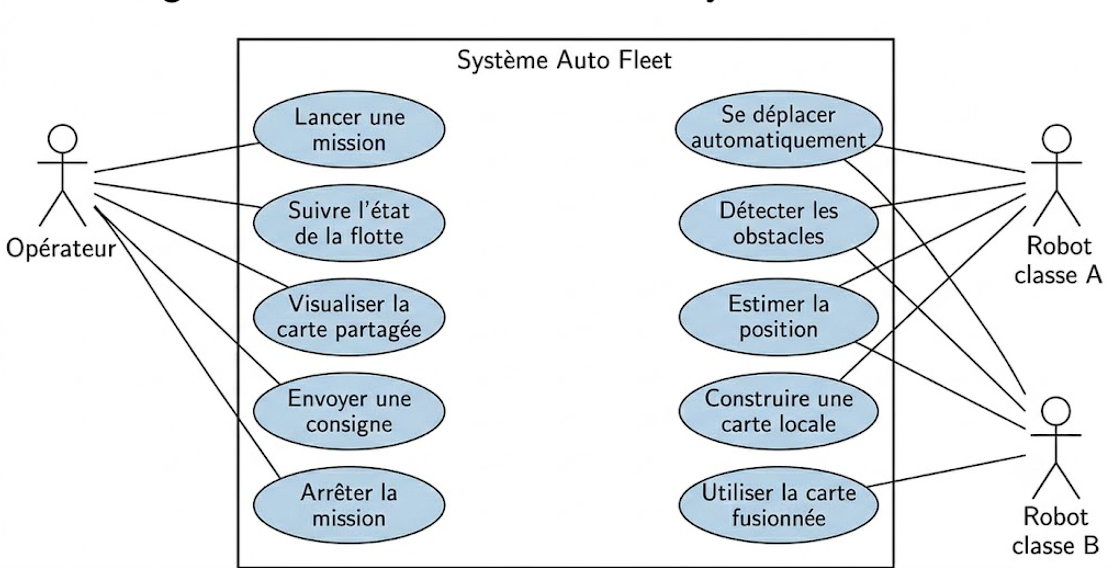
\includegraphics[width=0.9\textwidth]{images/UML.png}
    \caption{Diagramme de cas d’utilisation du système Auto Fleet}
    \label{fig:use_case_auto_fleet}
\end{figure}

\subsection*{Structure du rapport}
\addcontentsline{toc}{subsection}{Structure du rapport}

Afin d’éviter une lecture morcelée, le rapport est organisé selon une progression qui va du \kw{cadre général} vers les \kw{couches techniques}, puis vers les éléments de \kw{validation} et de \kw{gestion de projet}. Cette structuration n’a pas été pensée comme un simple enchaînement rédactionnel ; elle reflète l’ordre logique selon lequel les choix techniques deviennent intelligibles.

\begin{itemize}[leftmargin=1.2cm]
    \item \kw{Chapitre 2 --- Conception et vue globale du projet.}  
    Ce chapitre a pour fonction de fixer le \kw{socle architectural} du système. Il présente la logique distribuée retenue, la séparation entre fonctions embarquées et supervision, ainsi que l’environnement de développement qui a permis d’itérer sur le projet. L’enjeu de ce chapitre n’est pas encore d’entrer dans le détail composant par composant, mais de poser la lecture d’ensemble : quels sont les blocs du système, comment circulent les données, quelles briques logicielles ont été mobilisées et selon quel découpage fonctionnel la flotte est structurée. Il sert également de point d’ancrage pour les chapitres suivants, en explicitant les choix de base qui justifient à la fois la conception matérielle, la perception, la communication et la supervision.

    \item \kw{Chapitre 3 --- Architecture embarquée des robots autonomes.}  
    Ce chapitre constitue le noyau matériel du rapport. Il traite des \kw{contraintes fonctionnelles}, des \kw{contraintes mécaniques}, des limites d’\kw{alimentation}, du découpage entre calcul haut niveau et commande temps réel, ainsi que de l’intégration effective des composants sur les plateformes. Une attention particulière y est portée à la notion d’\kw{architecture distribuée embarquée}, indispensable dès lors qu’un système Linux généraliste ne peut suffire à garantir seul les exigences de réactivité des boucles moteur. Le chapitre documente aussi la phase d’intégration, c’est-à-dire le moment où les hypothèses théoriques rencontrent les réalités du câblage, des vibrations, des chutes de tension, des synchronisations temporelles et des compromis d’encombrement. Enfin, il ouvre naturellement sur la question du \kw{SLAM collaboratif}, en montrant que la cartographie ne peut être dissociée de la stabilité de l’architecture physique qui la supporte.

    \item \kw{Chapitre 4 --- Perception de l’environnement par capteurs embarqués.}  
    La perception n’est pas traitée ici comme un module accessoire. Elle constitue la condition d’existence même de l’autonomie. Ce chapitre expose les besoins de captation du projet, justifie le choix des capteurs, discute leurs limites respectives et formalise la manière dont leurs données sont acquises, filtrées, fusionnées et exploitées. Il montre en particulier pourquoi une approche mono-capteur serait insuffisante dans le cadre d’une flotte évoluant en environnement partiellement inconnu. Le lecteur y trouvera les éléments nécessaires pour comprendre la production de l’odométrie, l’estimation d’état, l’appui du \kw{LiDAR} sur la cartographie, le rôle de l’\kw{IMU} dans la stabilité des estimations, ainsi que la contribution de la \kw{caméra} et des capteurs de proximité à la robustesse globale du système. Ce chapitre prépare également l’analyse critique des performances observées en conditions réelles.

    \item \kw{Chapitre 5 --- Communication entre robots et supervision.}  
    Ce chapitre se concentre sur la \kw{chaîne V2X} au sens large : échanges entre robots, backend, broker de messages et interface opérateur. Il ne se limite pas à décrire une pile de communication ; il interroge la place de la supervision dans un système qui, par principe, doit conserver une part d’autonomie locale. Les différents types de messages y sont distingués selon leur criticité, leur fréquence et leur charge potentielle sur le réseau. La logique de l’\kw{IHM} y est également abordée sous un angle fonctionnel : il s’agit moins de détailler une interface écran par écran que de montrer comment sont articulés \kw{contrôle}, \kw{visibilité du système}, \kw{diagnostic réseau}, \kw{accès vidéo} et \kw{retours de mission}. Ce chapitre a enfin une dimension évaluative, puisqu’il introduit les métriques de qualité de service utiles pour juger la stabilité réelle de la supervision.

    \item \kw{Chapitre 6 --- Rendu final.}  
    Ce chapitre est volontairement orienté vers la \kw{présentation consolidée du prototype}. Il accueillera les éléments démontrables du système : organisation finale de l’interface, interactions réellement exposées à l’utilisateur, scénarios de test retenus et résultats visibles depuis le point de vue opérateur. Sa fonction n’est pas de répéter les détails d’architecture déjà exposés, mais de rendre compte de ce qui est effectivement stabilisé au moment de la démonstration. Il s’agit donc d’un chapitre de \kw{synthèse opérationnelle}, où devront converger les choix de conception, les campagnes de tests et les contraintes réellement surmontées dans la version présentée.

    \item \kw{Chapitre 7 --- Gestion de projet.}  
    La cohérence d’Auto Fleet ne peut être comprise sans un retour explicite sur l’organisation du travail. Ce chapitre documente la méthode adoptée, la répartition des responsabilités, les ajustements imposés par les retards matériels, le rôle joué par la simulation lorsqu’une partie de l’intégration réelle demeurait incomplète, ainsi que les outils de coordination mobilisés par l’équipe. Il ne s’agit pas d’un ajout périphérique : dans un projet à forte composante d’intégration, la gestion de projet influence directement les choix techniques, les priorités de développement et le rythme de validation des briques critiques. Ce chapitre permet donc de rendre lisible la manière dont les décisions ont été arbitréés, révisées et, parfois, contraintes par les réalités du calendrier et de l’approvisionnement.

    \item \kw{Chapitre 8 --- Conclusion et perspectives.}  
    Le dernier chapitre clôt le rapport par une synthèse des résultats atteints, des verrous demeurant ouverts et des prolongements techniquement crédibles. Il doit permettre de distinguer ce qui relève d’une \kw{preuve de faisabilité}, ce qui relève d’un \kw{prototype partiellement stabilisé} et ce qui constitue encore une \kw{perspective de développement}. Cette conclusion ne vise pas à produire une clôture rhétorique ; elle doit au contraire laisser apparaître les marges d’amélioration concernant la perception, la cartographie, la robustesse réseau, la compacité embarquée et la montée en échelle du système.
\end{itemize}

% =========================
% CHAPITRE 2
% =========================
\chapter{Conception et vue globale du projet}

Ce chapitre fixe le cadre architectural d’Auto Fleet. Il établit les choix de séparation fonctionnelle, introduit les sous-systèmes majeurs et précise l’environnement technique ayant servi au développement.

\section{Architecture technique globale}

L’architecture du projet repose sur une logique \kw{distribuée}, \kw{modulaire} et \kw{partiellement hétérogène}. Chaque robot conserve des capacités de décision locale, tandis qu’une partie des informations utiles à la mission est remontée, consolidée ou redistribuée à l’échelle de la flotte.

\subsection{Vue d’ensemble du système}

Auto Fleet est conçu comme un système dans lequel plusieurs robots mobiles autonomes opèrent dans un même environnement tout en conservant un degré significatif d’autonomie locale. Chaque unité embarque des capteurs, une puissance de calcul, une chaîne de commande moteur, une alimentation et des capacités de communication lui permettant de traiter son état immédiat sans dépendre en permanence d’un poste central.

L’architecture générale repose sur une séparation entre plusieurs couches fonctionnelles. La première couche correspond à la \kw{perception embarquée} : acquisition de distances, d’images, d’informations inertielles et de données de déplacement. La deuxième couche relève du \kw{traitement local} : filtrage, estimation d’état, détection d’événements, préparation de commandes et mise en forme des informations à transmettre. La troisième couche est celle de la \kw{commande}, chargée de convertir les décisions de haut niveau en signaux effectivement utilisables par les actionneurs.

La flotte n’est pas strictement homogène. Deux robots sont équipés d’un \kw{LiDAR LD06} et participent directement à la \kw{cartographie} de l’environnement. Les deux autres utilisent principalement une \kw{caméra} et leur perception locale pour l’exploration et la progression. Cette dissymétrie fonctionnelle est volontaire : elle permet de mieux répartir les rôles, de limiter le surcoût matériel et de faire émerger une logique de coopération plutôt qu’une simple duplication de plateformes identiques.

Dans cette architecture, la station de supervision ne remplace pas la décision embarquée. Elle fournit une vue consolidée de la mission, centralise certains états, transmet des consignes et rend observables les résultats de la mission. Le système doit donc être lu comme un ensemble dans lequel \kw{autonomie locale} et \kw{supervision globale} coexistent sans s’annuler.

\subsection{Sous-systèmes embarqués des robots}

Les robots embarquent plusieurs sous-systèmes complémentaires dont l’agencement conditionne la cohérence de l’ensemble.

Le premier sous-système est la \kw{chaîne de perception}. Elle comprend, selon les robots, une \kw{caméra}, un \kw{LiDAR}, une \kw{IMU}, des \kw{encodeurs} et des capteurs de proximité. Cette chaîne n’a pas pour seule fonction de détecter des obstacles : elle soutient aussi l’odométrie, la localisation, la navigation et, pour les robots concernés, la production d’une carte exploitable.

Le second sous-système est le \kw{calcul embarqué}. Une carte principale exécute les fonctions de plus haut niveau : lecture des capteurs, préparation des échanges \outil{ROS 2}, estimation d’état, supervision locale, traitement des consignes et, le cas échéant, exécution des briques de \kw{SLAM}. Cette couche est le centre de décision logiciel du robot.

Le troisième sous-système est la \kw{commande bas niveau}. Il regroupe un microcontrôleur, les drivers moteurs et les boucles d’asservissement nécessaires à la production d’un comportement mécanique stable. Ce découplage entre traitement haut niveau et commande temps réel n’est pas un luxe d’implémentation ; il répond à une contrainte de réactivité que la carte principale ne peut garantir seule dans toutes les situations.

Enfin, un dernier sous-système couvre la \kw{communication} et la \kw{gestion énergétique}. Les modules réseau assurent la circulation des états et des consignes, tandis que la distribution électrique doit satisfaire des profils de consommation très différents entre capteurs, calcul embarqué et actionneurs.

\begin{figure}[H]
    \centering
    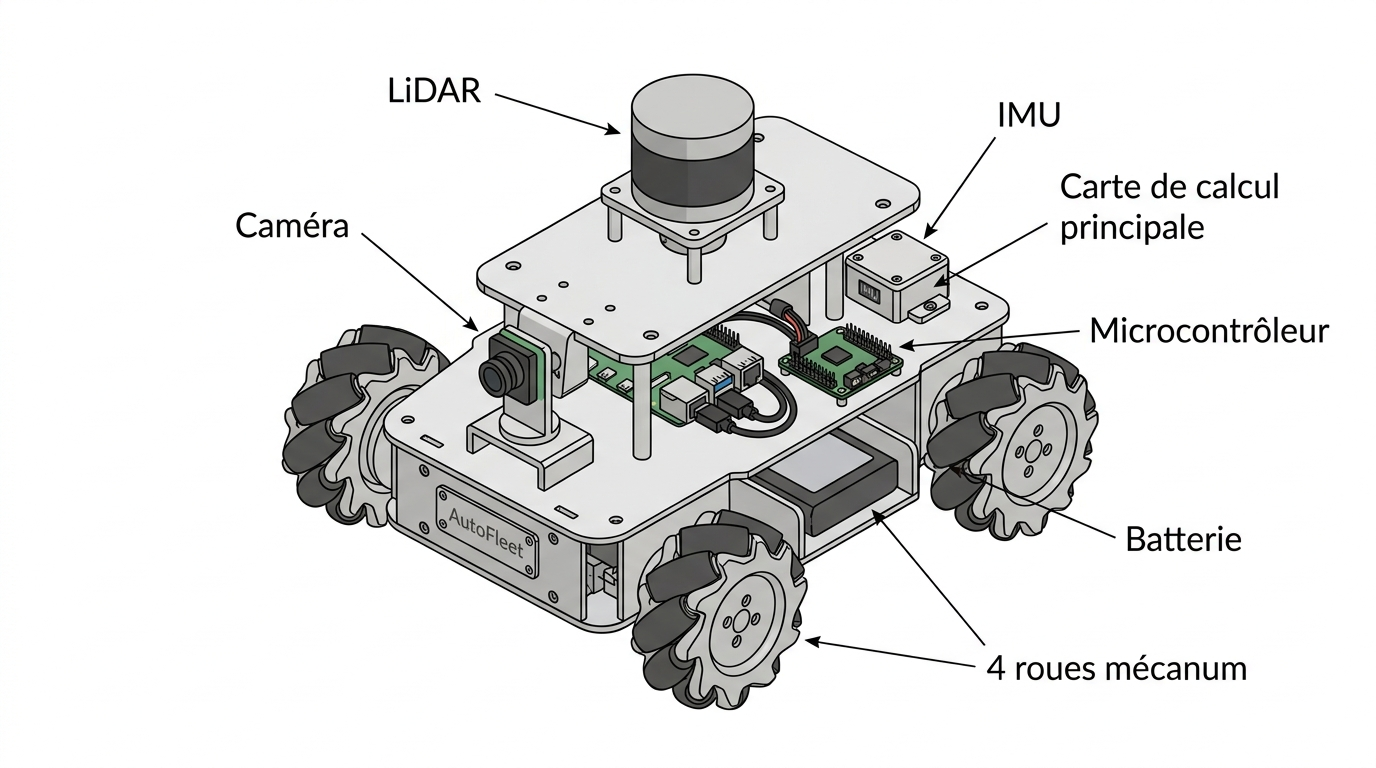
\includegraphics[width=0.92\textwidth]{images/archi_generale.png}
    \caption{Architecture embarquée type d’un robot de la flotte Auto Fleet}
    \label{fig:archi_generale_robot}
\end{figure}

\subsection{Communication et supervision de la flotte}

Au-delà du fonctionnement local des robots, Auto Fleet intègre une couche de communication chargée de relier la flotte à une station de supervision. Cette couche transporte des \kw{commandes}, des \kw{états}, de la \kw{télémétrie}, des \kw{événements de mission} et, pour les robots équipés en \kw{LiDAR}, des informations utiles à la \kw{cartographie partagée}.

Les échanges servent d’abord à rendre le système observable. Sans cette remontée d’informations, l’opérateur ne disposerait que d’une perception fragmentaire de la mission. Ils servent ensuite à rendre le système pilotable à un niveau supérieur : lancement d’une mission, arrêt d’un robot, modification d’un mode de fonctionnement ou suivi de l’état global de la flotte.

L’architecture de supervision retenue conserve néanmoins un principe important : la sécurité immédiate et la navigation de proximité restent \kw{embarquées}. Ainsi, une dégradation temporaire du lien réseau ne doit pas suffire à placer un robot dans un état incontrôlé. La supervision complète l’autonomie ; elle ne s’y substitue pas.

\section{Environnement de développement du projet}

Le développement d’Auto Fleet a nécessité un environnement de travail capable d’articuler \kw{simulation}, \kw{programmation embarquée}, \kw{intégration matérielle} et \kw{travail collaboratif}. L’intérêt de cet environnement est moins la diversité des outils que la cohérence de leur usage.

\subsection{Outils logiciels utilisés}

Le développement logiciel s’appuie sur plusieurs ensembles d’outils, chacun correspondant à un niveau distinct du système.

Les fonctions de bas niveau et les interfaces matérielles critiques sont principalement implémentées en \kw{C/C++}, afin de conserver une maîtrise suffisante du matériel, des temps d’exécution et de l’accès direct aux périphériques. Cette couche est particulièrement pertinente pour la commande moteur, la lecture d’encodeurs, les échanges série et les routines proches du temps réel.

Les développements nécessitant davantage de flexibilité reposent sur \outil{Python}. Ce langage a été retenu pour le prototypage rapide, l’outillage interne, certains scripts de test, la manipulation de données capteurs et certaines briques associées à la supervision. Dans ce cadre, la rapidité d’itération et la lisibilité priment sur l’optimisation basse couche.

La colonne vertébrale logicielle du projet demeure \outil{ROS 2}. Ce middleware structure les échanges internes au robot et, selon les cas, entre plusieurs nœuds répartis sur le réseau local. Des outils comme \outil{RViz 2} sont mobilisés pour la visualisation, tandis que les briques de cartographie s’appuient notamment sur \texttt{slam\_toolbox}. L’objectif n’est pas d’empiler des logiciels, mais de construire une chaîne de traitement intelligible, déboguable et progressive.

\subsection{Environnement matériel et simulation}

Le développement d’Auto Fleet repose sur une approche hybride combinant \kw{plateformes réelles} et \kw{simulation}. Ce choix n’a pas été dicté par confort méthodologique mais par nécessité d’intégration : plusieurs briques pouvaient être validées en simulation alors que le matériel complet n’était pas encore stabilisé.

Le banc d’essai réel est constitué de quatre robots mobiles embarquant une \kw{Raspberry Pi 5}, un microcontrôleur \kw{ESP32}, des moteurs DC encodés, une \kw{caméra NoIR}, une \kw{IMU}, un \kw{LiDAR LD06} pour les robots instrumentés, ainsi qu’une alimentation sur batterie de type \kw{LiPo 3S}. Cette plateforme permet de confronter les hypothèses de conception aux contraintes effectives d’intégration : qualité réelle des mesures, latence des échanges, sensibilité aux vibrations, tenue de l’alimentation et comportement dynamique des châssis.

En parallèle, la simulation a joué un rôle structurant. \outil{Gazebo Sim} a été utilisé pour modéliser les robots et certaines interactions physiques, \outil{RViz 2} pour visualiser les cartes et la télémétrie, et \outil{ROS 2} pour exécuter les nœuds de perception, de navigation et de communication sur une architecture distribuée. La simulation a surtout servi à réduire le coût des itérations logicielles, à éprouver la cohérence des flux de données et à préparer les campagnes d’intégration matérielle.

L’intérêt de cette double approche est concret : elle permet de dissocier, autant que possible, les erreurs de logique algorithmique des défauts d’intégration physique. En pratique, la simulation n’annule pas la nécessité des essais réels ; elle permet simplement d’arriver à ces essais avec des hypothèses déjà filtrées.

\subsection{Outils de collaboration et de gestion de version}

Le travail collectif ne repose pas sur un outil unique, mais sur un petit ensemble d’outils complémentaires.

Le versionnage du code est assuré par \outil{Git}. Son usage ne se limite pas à la conservation d’un historique : il structure les branches de développement, facilite l’isolation des modifications risquées, rend les retours en arrière traçables et permet de distinguer plus proprement les phases d’expérimentation des versions plus stables.

Ce dépôt est associé à une \kw{forge distante}, utilisée pour centraliser les branches de travail, gérer les intégrations successives et conserver une trace des arbitrages techniques. La dimension collaborative ne se réduit donc pas à « partager des fichiers » ; elle implique aussi de rendre visibles les conflits, les fusions, les dépendances et la chronologie des décisions.

En complément, un espace de \kw{partage documentaire} regroupe les schémas, comptes rendus, références techniques et ressources communes du projet. Des canaux de \kw{messagerie d’équipe} et, lorsque nécessaire, des outils simples de \kw{suivi de tâches} ont servi à coordonner les tests, à signaler les anomalies et à répartir le travail sans laisser se multiplier des versions concurrentes d’un même sous-système. Le recours à plusieurs outils se justifie ici pleinement : le pluriel du titre renvoie à des besoins distincts, et non à une simple redondance terminologique.

Le \kw{Tableau~\ref{tab:problematiques_techniques}} synthétise les principales problématiques techniques traitées dans le projet et les orientations retenues pour y répondre.

\begin{table}[H]
\centering
\renewcommand{\arraystretch}{1.35}
\begin{tabular}{|p{5cm}|p{10cm}|}
\hline
\textbf{Problématique technique} & \textbf{Solution envisagée dans le projet} \\
\hline
\kw{Déplacement autonome} & Utilisation d'une commande moteur bas niveau associée à une logique de navigation embarquée \\
\hline
\kw{Perception de l'environnement} & Combinaison de plusieurs capteurs : \kw{LiDAR}, \kw{caméra}, \kw{IMU}, \kw{encodeurs} et capteurs de proximité \\
\hline
\kw{Cartographie partagée} & Mise en place d'une approche de \kw{SLAM} sur les robots équipés d'un \kw{LiDAR}, avec fusion des cartes partielles \\
\hline
\kw{Communication de la flotte} & Utilisation d'échanges réseau entre robots, backend et station de supervision \\
\hline
\kw{Supervision utilisateur} & Développement d'une interface graphique permettant de visualiser l'état des robots et l'évolution de la mission \\
\hline
\end{tabular}
\caption{Principales problématiques techniques du projet Auto Fleet}
\label{tab:problematiques_techniques}
\end{table}

% =========================
% CHAPITRE 3
% =========================
\chapter{Architecture embarquée des robots autonomes}

L’architecture embarquée est ici considérée comme un problème d’intégration complet. Elle engage à la fois la structure mécanique, la distribution d’énergie, l’organisation des calculs, la commande des actionneurs et la capacité du système à rester stable lorsqu’il est effectivement mis en mouvement.

\section{Contraintes et besoins de l'architecture embarquée}

L’identification des contraintes est un préalable nécessaire à tout choix de composants. Une architecture embarquée n’est pas seulement une juxtaposition d’éléments compatibles ; c’est un compromis entre fonctions attendues, limites physiques, exigences de sûreté et capacité réelle d’intégration.

\subsection{Besoins fonctionnels des robots}

Les besoins fonctionnels des robots ne se limitent pas à la locomotion. Chaque plateforme doit fonctionner comme un \kw{nœud autonome de traitement} capable d’assurer simultanément la perception de son environnement, l’estimation de son état, l’exécution de consignes, la remontée d’informations vers la supervision et le maintien d’un comportement sûr en cas de dégradation partielle d’un composant logiciel ou réseau.

La flotte repose sur une \kw{hétérogénéité maîtrisée}. Deux robots, désignés comme \kw{classe A}, embarquent un \kw{LiDAR LD06}, une \kw{IMU} et une base roulante à roues mécanum. Ils sont prioritairement mobilisés pour la \kw{perception géométrique} de l’environnement, la \kw{localisation} et la \kw{cartographie}. Deux autres robots, dits \kw{classe B}, disposent principalement d’une \kw{caméra NoIR}, d’une architecture plus légère et d’un rôle davantage centré sur l’exploration, le déplacement et l’exploitation de données déjà consolidées à l’échelle de la flotte.

Ce découpage répond à une contrainte simple : il n’est ni nécessaire ni souhaitable que chaque robot embarque l’ensemble des capteurs et traitements les plus coûteux. Une flotte efficace ne suppose pas l’uniformité complète ; elle suppose plutôt une répartition des fonctions permettant d’optimiser \kw{coût}, \kw{masse}, \kw{consommation} et \kw{charge de calcul}. Les robots de classe A produisent l’information la plus structurée sur l’environnement, tandis que les robots de classe B peuvent en bénéficier sans supporter la totalité du coût matériel associé.

Sur le plan logiciel, l’architecture s’appuie sur \outil{ROS 2}. Les fonctions sont organisées en nœuds distincts : perception, odométrie, commande, navigation, cartographie, communication et supervision. Cette structuration favorise le découplage des responsabilités et permet une évolution plus propre des sous-systèmes. Les échanges s’appuient sur des topics, des messages horodatés et un modèle de communication cohérent avec les besoins d’une architecture distribuée.

Les robots de classe A exécutent localement une chaîne de \kw{SLAM}, par exemple via \texttt{slam\_toolbox}. Ils produisent une carte locale à partir des scans \kw{LiDAR} et de l’odométrie enrichie. Cette carte est ensuite transmise au poste de supervision, où peut être réalisée une opération de fusion lorsqu’un recouvrement suffisant existe entre les zones explorées. Les robots de classe B n’exécutent pas cette chaîne complète ; ils peuvent toutefois exploiter les informations consolidées à l’échelle globale.

La communication repose principalement sur le \kw{Wi-Fi} embarqué des \kw{Raspberry Pi}. Grâce au middleware \kw{DDS} de \outil{ROS 2}, la communication interne au système conserve une logique décentralisée. Cette propriété est importante : elle évite qu’un unique point logique ne devienne un goulot d’étranglement pour les échanges de perception et d’état.

Enfin, l’architecture doit rester \kw{évolutive}. Le projet ne vise pas un robot figé, mais une plateforme susceptible d’accueillir des améliorations progressives. Cela impose de préserver des interfaces claires entre les modules et de limiter les dépendances excessivement serrées entre perception, commande, communication et supervision.

\subsection{Contraintes mécaniques et énergétiques}

Les choix techniques sont fortement contraints par le châssis, l’encombrement disponible, la masse embarquée et la distribution de puissance. Même lorsqu’une solution paraît satisfaisante sur le plan fonctionnel, elle peut devenir inexploitablesi son intégration physique dégrade la stabilité du robot ou la qualité des mesures.

Chaque plateforme doit accueillir, dans un volume restreint, une carte de calcul, un microcontrôleur, les drivers moteurs, des capteurs, une batterie et l’ensemble du câblage associé. Cette contrainte impose une implantation rigoureuse. Les éléments qui font l’objet de manipulations fréquentes  batterie, connecteurs d’alimentation, liaisons série, drivers  doivent rester accessibles afin de rendre les tests et la maintenance possibles.

Les robots de classe A sont mécaniquement les plus contraints en raison de la présence du \kw{LiDAR}. Le capteur doit être placé de manière à préserver un champ de vue dégagé à 360 degrés. Une obstruction partielle dans le plan de balayage introduirait des zones aveugles et dégraderait directement la qualité de la carte produite. En outre, le support du capteur doit limiter les vibrations, car une mesure géométriquement précise perd rapidement de sa valeur lorsqu’elle est portée par une structure instable.

Le choix de roues mécanum implique également une géométrie suffisamment rigoureuse. Un mauvais alignement, une dissymétrie d’empattement ou une répartition de masse défavorable peuvent introduire des comportements parasites : glissement accru, rotations non désirées, dérive de trajectoire ou dégradation de l’odométrie.

La contrainte énergétique est tout aussi structurante. La batterie retenue est une \kw{LiPo 3S 5200 mAh}, de tension nominale \(11{,}1\,V\). Les moteurs et leurs drivers peuvent être alimentés à partir de cette source, tandis qu’un convertisseur \kw{DC-DC} abaisseur fournit le \(5\,V\) stabilisé nécessaire à la \kw{Raspberry Pi} et aux périphériques basse tension.

Le \kw{Tableau~\ref{tab:consommation_classes}} propose une estimation des puissances en jeu pour les deux classes de robots. Ces valeurs restent nécessairement indicatives : la consommation réelle dépend de la charge processeur, du nombre de capteurs actifs, du profil d’accélération et du type de manœuvre demandé.

\begin{table}[H]
\centering
\small
\begin{tabular}{|p{4.8cm}|p{2.6cm}|p{2.4cm}|p{2.3cm}|c|c|}
\hline
\textbf{Composant} & \textbf{Tension} & \textbf{Courant typique} & \textbf{Puissance} & \textbf{A} & \textbf{B} \\
\hline
Raspberry Pi 5 8 Go & 5 V & 3 à 5 A & 15 à 25 W & Oui & Oui \\
\hline
ESP32 & 3,3 V & $\approx 0,24$ A & $\approx 0,8$ W & Oui & Oui \\
\hline
LiDAR LD06 & 5 V & $\approx 0,5$ A & $\approx 2,5$ W & Oui & Non \\
\hline
IMU 6 axes & 3,3 V & $\approx 3,9$ mA & $\approx 0,013$ W & Oui & Non \\
\hline
RaspiCam V3 NoIR & 3,3 V & $\approx 0,25$ A & $\approx 0,8$ W & Oui & Oui \\
\hline
4 moteurs DC encodés & 7,4 à 12 V & $\approx 1$ A/moteur & $\approx 16$ W & Oui & Oui \\
\hline
Drivers moteurs & -- & -- & $\approx 1$ W & Oui & Oui \\
\hline
Convertisseur DC-DC & -- & -- & pertes $\approx 12\,\%$ & Oui & Oui \\
\hline
\textbf{Puissance totale estimée} & -- & -- & \textbf{$\approx 63$ W / $59$ W} & \textbf{A} & \textbf{B} \\
\hline
\end{tabular}
\caption{Estimation de la consommation électrique des robots de classe A et B}
\label{tab:consommation_classes}
\end{table}

La capacité énergétique utilisable de la batterie peut être estimée par :
\[
E_{utile} = V_{nom} \times C_{bat} \times \eta_{\mathrm{decharge}}
\]

avec \(V_{nom}=11{,}1\,V\), \(C_{bat}=5{,}2\,Ah\) et un rendement de décharge estimé à \(\eta_{\mathrm{decharge}}=0{,}85\). On obtient :
\[
E_{utile} = 11{,}1 \times 5{,}2 \times 0{,}85 \approx 49\,Wh
\]

L’autonomie théorique devient alors :
\[
t_A = \frac{49}{63} \approx 47\,min
\qquad
t_B = \frac{49}{59} \approx 50\,min
\]

Ces valeurs constituent une borne haute. En conditions réelles, les transitoires de courant, les rotations, les déplacements latéraux et les charges CPU élevées réduisent sensiblement l’autonomie exploitable. Une durée de fonctionnement utile de l’ordre de \kw{35 à 40 minutes} paraît plus réaliste dans un scénario de mission continue.

\subsection{Choix d'une architecture embarquée distribuée}

Au regard des contraintes précédentes, une architecture embarquée à \kw{deux niveaux de calcul} a été retenue.

Le \kw{niveau supérieur} est assuré par une \kw{Raspberry Pi 5}. Il prend en charge les fonctions de traitement non strictement déterministes : exécution des nœuds \outil{ROS 2}, acquisition capteurs, fusion de données, logique de navigation, communication réseau, supervision locale et, pour les robots de classe A, traitement du \kw{SLAM}. Ce niveau requiert une puissance de calcul significative, mais n’a pas vocation à assurer seul les boucles d’asservissement les plus rapides.

Le \kw{niveau inférieur} est assuré par un \kw{ESP32}. Ce microcontrôleur exécute les tâches les plus proches du temps réel : génération des signaux \kw{PWM}, lecture des encodeurs, boucles \kw{PID} de vitesse et mécanismes de sécurité élémentaires. Cette séparation n’est pas seulement commode ; elle répond à une nécessité pratique. Un système Linux généraliste offre de la souplesse, mais ne garantit pas, à lui seul, une régularité suffisante pour des boucles de commande moteurs exigeantes.

La communication entre les deux niveaux peut s’effectuer via \kw{UART} ou \kw{SPI}. Les messages transportent typiquement des consignes de vitesse, des états moteurs, des mesures d’encodeurs ou des informations d’odométrie. Cette liaison doit rester simple, robuste et suffisamment rapide pour ne pas dégrader la fréquence effective de commande.

L’intérêt de cette architecture réside également dans sa \kw{robustesse fonctionnelle}. En cas de défaillance partielle du traitement haut niveau, le microcontrôleur peut imposer un état sûr, par exemple l’arrêt des moteurs en l’absence de commande valide sur un intervalle défini. La chaîne de commande ne dépend donc pas complètement de l’état instantané de la carte principale.

% =========================
% SECTION 3.2
% =========================
\section{Conception matérielle et intégration des robots}

Cette section détaille la mise en œuvre matérielle de l’architecture retenue. Elle traite à la fois de la structure physique des plateformes et des flux effectifs traversant les composants embarqués.

\subsection{Structure mécanique et châssis}

Le châssis constitue l’ossature physique de chaque robot. Il ne s’agit pas d’un simple support, mais d’un élément déterminant pour la stabilité mécanique, l’accessibilité des composants et la qualité finale des mesures.

Pour les robots de classe A, l’usage de roues mécanum impose une géométrie rectangulaire et une implantation suffisamment symétrique. La cinématique inverse d’une base à quatre roues peut s’écrire sous la forme :

\[
\begin{pmatrix}
\omega_{FL} \\
\omega_{FR} \\
\omega_{RL} \\
\omega_{RR}
\end{pmatrix}
=
\frac{1}{r}
\begin{pmatrix}
1 & -1 & -(L+W) \\
1 & 1 & (L+W) \\
1 & 1 & -(L+W) \\
1 & -1 & (L+W)
\end{pmatrix}
\begin{pmatrix}
v_x \\
v_y \\
\omega_z
\end{pmatrix}
\]

où \(r\) représente le rayon des roues, \(L\) le demi-empattement longitudinal, \(W\) le demi-empattement latéral, \(v_x\) et \(v_y\) les vitesses linéaires dans le repère du robot, et \(\omega_z\) la vitesse de rotation autour de l’axe vertical.

Les notations de cette matrice sont rappelées dans le \kw{Tableau~\ref{tab:variables_mecanum}}. Cette explicitation est utile, car le passage d’un modèle cinématique à une implémentation embarquée est une source fréquente d’ambiguïtés si les conventions géométriques ne sont pas strictement posées.

\begin{table}[H]
\centering
\renewcommand{\arraystretch}{1.2}
\begin{tabular}{|p{2.5cm}|p{8.3cm}|p{2.2cm}|}
\hline
\textbf{Symbole} & \textbf{Signification} & \textbf{Unité} \\
\hline
\(r\) & Rayon d’une roue & m \\
\hline
\(L\) & Demi-empattement longitudinal & m \\
\hline
\(W\) & Demi-empattement latéral & m \\
\hline
\(v_x\) & Vitesse longitudinale du robot & m/s \\
\hline
\(v_y\) & Vitesse latérale du robot & m/s \\
\hline
\(\omega_z\) & Vitesse angulaire autour de l’axe vertical & rad/s \\
\hline
\(\omega_{FL}, \omega_{FR}, \omega_{RL}, \omega_{RR}\) & Vitesses angulaires des roues avant gauche, avant droite, arrière gauche et arrière droite & rad/s \\
\hline
\end{tabular}
\caption{Signification des variables de la matrice cinématique des roues mécanum}
\label{tab:variables_mecanum}
\end{table}

Ce modèle montre immédiatement qu’une erreur mécanique sur \(L\), \(W\) ou sur l’alignement des roues se répercute sur la qualité de la commande et, par conséquent, sur l’odométrie. Dans une plateforme omnidirectionnelle, cette sensibilité est plus marquée que sur une base différentielle classique.

La répartition des masses a également été traitée comme un point critique. La batterie, qui constitue l’un des éléments les plus lourds, est positionnée au plus près du centre du châssis afin de limiter les déséquilibres dynamiques. Cette disposition améliore particulièrement le comportement lors des translations latérales et des rotations rapides.

Pour les robots équipés d’un \kw{LiDAR}, le support mécanique du capteur doit à la fois dégager le plan de balayage et limiter les vibrations. Une fixation insuffisamment rigide dégrade directement la qualité des scans et, par conséquent, celle du \kw{SLAM}. Dans la pratique, plusieurs ajustements de positionnement ont été nécessaires avant d’obtenir une implantation satisfaisante.

\subsection{Capteurs, cartes embarquées et actionneurs}

L’architecture matérielle se compose de plusieurs familles de composants : \kw{capteurs}, \kw{cartes de calcul}, \kw{actionneurs} et \kw{alimentation}.

Les robots de classe A embarquent un \kw{LiDAR LD06}. Ce capteur réalise un balayage 2D à \(360^\circ\), adapté à la détection d’obstacles et à la production de cartes d’occupation. Sa fréquence de rotation et sa compacité en font un choix cohérent pour une plateforme mobile de taille réduite.

Une \kw{IMU 6 axes} fournit des mesures d’accélération et de vitesse angulaire. Isolément, ce capteur ne suffit pas à assurer une localisation fiable sur longue durée ; en revanche, il constitue une source précieuse pour améliorer l’estimation d’orientation et compenser partiellement certaines dérives d’odométrie sur des horizons temporels courts.

La \kw{RaspiCam V3 NoIR} ajoute une perception visuelle de l’environnement. Dans l’état actuel du projet, cette caméra est principalement exploitée pour l’observation et l’exploration, mais elle constitue également un levier pour des développements ultérieurs en détection visuelle, suivi d’objets ou perception sémantique.

La \kw{Raspberry Pi 5} joue le rôle d’unité de calcul principale. Elle exécute les nœuds \outil{ROS 2}, les traitements capteurs, la logique de communication et, pour les robots de classe A, les briques de cartographie.

L’\kw{ESP32} assure la commande bas niveau. Il lit les encodeurs, applique les régulations \kw{PID}, génère les signaux \kw{PWM} et permet de conserver une commande moteur plus stable que si ces fonctions étaient laissées entièrement à la carte principale.

Chaque robot embarque quatre moteurs DC encodés. Les drivers de puissance, de type pont en H, pilotent les moteurs par paires. Cette organisation est bien adaptée à une base mobile à quatre roues et limite la complexité du câblage sans sacrifier la capacité de commande indépendante de chaque roue.

\subsection{Intégration des différents sous-systèmes}

L’intégration ne peut être réduite au montage physique des composants. Elle englobe aussi les connexions électriques, la hiérarchie des flux de données, les mécanismes d’horodatage et la distribution des responsabilités entre les différentes briques.

L’organisation retenue est centrée sur la \kw{Raspberry Pi}, qui collecte les données capteurs, exécute les traitements de haut niveau et transmet les consignes de déplacement à l’\kw{ESP32}. Celui-ci transforme ensuite ces consignes en commandes moteur et remonte les informations nécessaires à l’odométrie.

Le \kw{Tableau~\ref{tab:topics_ros2}} résume quelques flux \outil{ROS 2} représentatifs de l’architecture embarquée.

\begin{table}[H]
\centering
\small
\begin{tabular}{|p{3.2cm}|p{3.6cm}|p{3.2cm}|p{3.2cm}|p{1.8cm}|}
\hline
\textbf{Topic} & \textbf{Type} & \textbf{Émetteur} & \textbf{Récepteur} & \textbf{Fréquence} \\
\hline
\texttt{/robotN/scan} & \texttt{sensor\_msgs/LaserScan} & LiDAR LD06 & \texttt{slam\_toolbox} & 10 Hz \\
\hline
\texttt{/robotN/imu/data} & \texttt{sensor\_msgs/Imu} & IMU & Fusion capteurs & 100 Hz \\
\hline
\texttt{/robotN/odom} & \texttt{nav\_msgs/Odometry} & ESP32 / Raspberry Pi & SLAM, Nav2 & 50 Hz \\
\hline
\texttt{/robotN/map} & \texttt{nav\_msgs/OccupancyGrid} & \texttt{slam\_toolbox} & Supervision & 1 Hz \\
\hline
\texttt{/merged\_map} & \texttt{nav\_msgs/OccupancyGrid} & PC supervision & Robots, RViz 2 & 1 Hz \\
\hline
\texttt{/robotN/cmd\_vel} & \texttt{geometry\_msgs/Twist} & Nav2 / supervision & ESP32 & 20 Hz \\
\hline
\end{tabular}
\caption{Exemples de flux \outil{ROS 2} utilisés dans l’architecture embarquée}
\label{tab:topics_ros2}
\end{table}

Les robots de classe A produisent des données plus volumineuses et plus structurées, notamment les scans \kw{LiDAR} et les cartes locales. Ces données doivent être correctement horodatées afin de rester exploitables par les algorithmes de localisation et de cartographie. En pratique, l’horodatage côté \kw{Raspberry Pi} au moment de la réception des données issues de l’\kw{ESP32} permet de réduire certaines incohérences temporelles.

C’est également au niveau de l’intégration que les principales difficultés apparaissent : chutes de tension, câblage trop dense, bruit de mesure, vibrations, saturation partielle d’une liaison série ou désynchronisation entre sources. Le bon fonctionnement du système résulte donc autant de la qualité des choix matériels que de la manière dont ces éléments sont reliés et stabilisés dans le temps.

% =========================
% SECTION 3.3
% =========================
\section{Validation de l'architecture embarquée}

La validation de l’architecture embarquée ne se limite pas à constater qu’un robot se déplace. Elle consiste à vérifier que le système reste cohérent lorsqu’il exécute des trajectoires, alimente plusieurs sous-systèmes simultanément et transmet ses données sans dégradation excessive.

\subsection{Tests de locomotion et de commande moteur}

Les premières validations ont porté sur la chaîne de locomotion. Dans un premier temps, chaque moteur a été testé individuellement afin d’observer la réponse à une consigne et de régler les paramètres d’asservissement. La vitesse réelle estimée à partir des encodeurs a été comparée à la consigne injectée côté \kw{ESP32}. L’objectif n’était pas de produire une identification exhaustive mais de vérifier la stabilité de la réponse et l’absence d’écarts systématiques manifestes.

Dans un second temps, la cinématique globale de la plateforme a été éprouvée sur des mouvements élémentaires : translation avant, translation latérale, déplacement diagonal et rotation sur place. Ces essais permettent de vérifier la cohérence du modèle mécanum, le sens de rotation des roues et la qualité d’exécution des consignes coordonnées.

Sur un déplacement d’environ un mètre, une erreur finale de quelques centimètres reste observable. Cette dérive n’a rien d’anormal dans ce type de base roulante : elle provient des glissements, des imperfections mécaniques et des limites inhérentes au modèle d’odométrie. Les rotations révèlent également une sensibilité notable aux conditions d’adhérence.

Pour les robots de classe A, les essais de locomotion doivent être analysés conjointement avec la stabilité des mesures \kw{LiDAR}. Un déplacement mécaniquement correct mais produisant des scans instables reste problématique, car la qualité de la cartographie dépend directement de la tenue mécanique du capteur.

\subsection{Problèmes rencontrés lors de l'intégration}

Plusieurs difficultés sont apparues au cours de l’intégration.

La première est \kw{mécanique}. L’espace utile sur le châssis s’est révélé plus limité qu’anticipé, en particulier pour les robots intégrant un \kw{LiDAR}. L’implantation simultanée des cartes, des capteurs, des drivers, de la batterie et du câblage impose un arbitrage permanent entre accessibilité, stabilité et compacité.

La deuxième difficulté est \kw{électrique}. La \kw{Raspberry Pi 5} reste sensible aux chutes de tension, en particulier lors des appels de courant moteurs. Lorsque plusieurs roues accélèrent simultanément, des baisses transitoires du bus d’alimentation peuvent provoquer des sous-tensions, voire des redémarrages partiels de certains éléments.

La troisième difficulté est \kw{logicielle et temporelle}. Une liaison série sous-dimensionnée entre \kw{ESP32} et \kw{Raspberry Pi} peut devenir un facteur limitant dès lors que l’on souhaite transmettre non seulement les consignes, mais aussi l’odométrie, les états moteurs et les informations de diagnostic à fréquence soutenue.

Enfin, la fusion de cartes entre plusieurs robots met en évidence une difficulté d’un autre ordre : la cartographie collaborative dépend fortement de la qualité de l’odométrie, du recouvrement entre zones explorées et de la stabilité globale de l’architecture. Un problème matériel local peut donc réapparaître, plusieurs couches plus haut, sous la forme d’une incohérence cartographique.

\subsection{Ajustements et améliorations apportés}

Plusieurs corrections ont été introduites à la suite des difficultés précédentes.

Sur le plan électrique, des condensateurs de découplage ont été ajoutés sur le bus moteur afin d’atténuer les chutes de tension transitoires. Côté commande, une limitation du taux de variation des consignes a également été mise en œuvre sur l’\kw{ESP32} pour éviter les appels de courant trop abrupts.

Sur le plan mécanique, la batterie a été recentrée et les supports du \kw{LiDAR} ont été rigidifiés. Ces ajustements, bien que modestes en apparence, ont un effet direct sur la stabilité du robot et sur la qualité des données utilisées par le \kw{SLAM}.

Sur le plan logiciel, la liaison série a été accélérée et le protocole d’échange simplifié. À terme, un encodage binaire compact avec mécanisme élémentaire de contrôle d’intégrité pourrait encore améliorer la fiabilité des flux.

Enfin, l’usage du mode asynchrone de \texttt{slam\_toolbox} permet de maintenir une charge de calcul plus compatible avec la mobilité réelle du robot. Le choix réalisé ici est explicite : accepter un compromis mesuré sur la finesse de traitement afin de préserver la réactivité globale du système.

% =========================
% SECTION 3.4
% =========================
\section{SLAM collaboratif et cartographie partagée}

La cartographie collaborative prolonge naturellement l’architecture embarquée. Elle permet de passer d’une perception strictement locale à une représentation plus large de l’environnement, exploitable à l’échelle de la flotte et de la supervision.

\subsection{Problématique du SLAM multi-agents}

Le \kw{SLAM} --- \textit{Simultaneous Localization and Mapping} --- consiste à construire une carte tout en estimant la position du robot dans cette même carte. Dans Auto Fleet, cette difficulté est déplacée à une échelle supplémentaire : plusieurs robots peuvent produire, en parallèle, des cartes partielles qu’il faut ensuite rendre compatibles.

Deux robots de classe A, équipés d’un \kw{LiDAR LD06}, construisent chacun une carte locale. L’objectif n’est pas seulement de juxtaposer ces cartes, mais de les \kw{fusionner} dès lors qu’un recouvrement suffisant permet d’estimer une transformation cohérente entre leurs référentiels.

Le passage d’un \kw{SLAM mono-robot} à un \kw{SLAM multi-agents} introduit plusieurs contraintes nouvelles : maintien d’une cohérence de référentiel, gestion des délais de communication, qualité du recouvrement entre cartes, sensibilité accrue aux dérives d’odométrie et difficulté d’intégrer des observations partiellement asynchrones.

L’architecture logicielle retenue s’appuie principalement sur \texttt{slam\_toolbox} pour la construction locale des cartes, sur \texttt{multirobot\_map\_merge} pour la fusion et sur \texttt{explore\_lite} ou un équivalent pour l’exploration autonome.

\subsection{Exploration autonome par frontières}

L’exploration autonome repose sur le principe des \kw{frontières}, c’est-à-dire des zones situées à l’interface entre l’espace déjà connu comme libre et l’espace encore inconnu. Ce principe a l’avantage de fournir une heuristique simple, directement dérivable de la carte d’occupation.

À partir de la carte, l’algorithme détecte les groupes de cellules inconnues adjacentes à des cellules libres. Chaque frontière \(F_i\), composée de \(n_i\) cellules, peut être résumée par un centroïde :

\[
cent_i = \frac{1}{n_i}\sum_{j=1}^{n_i} f_{i,j}
\]

Un coût simple peut ensuite être défini :
\[
cost_i = \alpha \|cent_i - p\|_2 - \beta n_i
\]

où \(p\) désigne la position actuelle du robot. Le premier terme pénalise les frontières éloignées ; le second valorise celles dont la taille laisse espérer un gain informationnel plus important.

Cette approche est efficace mais imparfaite. Le centroïde d’une frontière n’est pas nécessairement atteignable et peut se trouver trop proche d’un obstacle ou dans une zone localement mal observée. Il doit donc être couplé à un planificateur de trajectoire, par exemple \kw{Nav2}, capable de vérifier la faisabilité du déplacement avant l’envoi effectif d’une consigne.

\subsection{Fusion des cartes partielles}

La fusion des cartes partielles est réalisée sur le poste de supervision. Le nœud \texttt{multirobot\_map\_merge} souscrit aux cartes locales publiées par les robots de classe A et produit une carte globale sur le topic \texttt{/merged\_map}.

Deux modes de fonctionnement peuvent être distingués. Dans le premier, les poses initiales des robots sont connues. L’algorithme de fusion part alors d’une estimation déjà raisonnable de la transformation entre cartes. Dans le second, ces poses ne sont pas connues et doivent être estimées à partir des zones de recouvrement détectées dans les cartes locales. Ce second cas est plus flexible mais également plus fragile.

Dans le cadre du projet, le mode avec \kw{poses initiales connues} est privilégié, car il réduit la complexité de la fusion et limite l’instabilité lorsque les cartes recouvrent mal les mêmes zones.

Pour une cellule donnée \((u,v)\), une règle probabiliste simple de fusion peut être écrite :
\[
P(M^*(u,v)=occupé)
=
1 -
\prod_{k \in \{1,2\}}
\left(
1 - P(M_k(T_k^{-1}(u,v))=occupé)
\right)
\]

Cette règle conserve un obstacle détecté par au moins une carte locale tout en maintenant l’état inconnu lorsqu’aucune observation n’est disponible. Elle constitue une solution simple, mais suffisante pour une première cartographie partagée.

\subsection{Architecture réseau et flux de données}

La flotte fonctionne sur un réseau \kw{Wi-Fi local}. Le poste de supervision centralise la visualisation, la fusion des cartes et une partie du suivi de mission. Toutefois, les échanges internes liés à la perception et à la navigation conservent la logique distribuée de \outil{ROS 2} et de \kw{DDS}.

\begin{figure}[H]
    \centering
    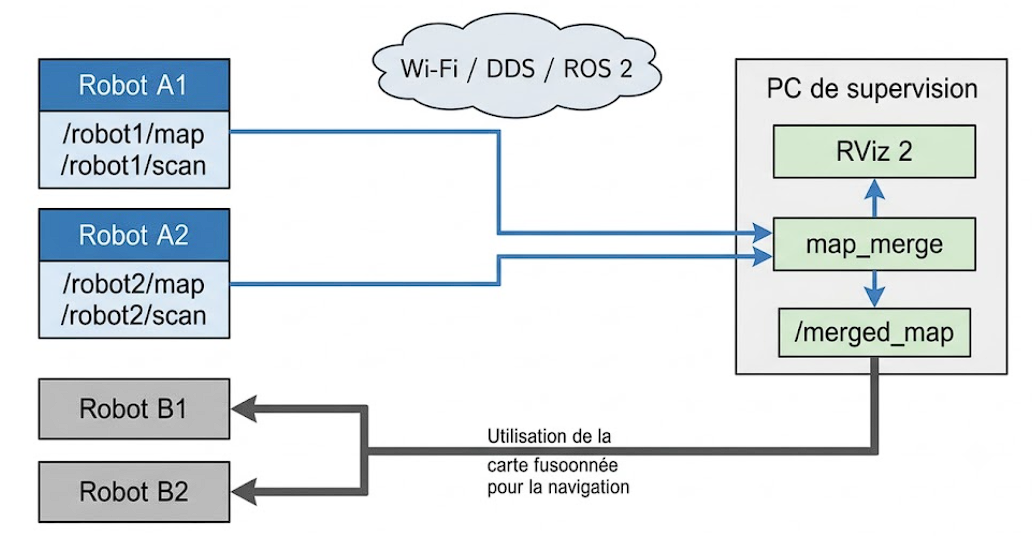
\includegraphics[width=0.9\textwidth]{images/ROS2.png}
    \caption{Flux de données associés à la cartographie partagée}
    \label{fig:ros2_map_flux}
\end{figure}

Les robots de classe A publient leurs cartes locales vers le poste de supervision. Celui-ci calcule une carte globale puis la republie sur \texttt{/merged\_map}. Les robots de classe B peuvent alors exploiter cette représentation commune sans embarquer eux-mêmes une chaîne complète de cartographie.

Le \kw{Tableau~\ref{tab:bande_passante_classe_a}} donne un ordre de grandeur de la bande passante consommée par quelques flux typiques d’un robot de classe A.

\begin{table}[H]
\centering
\small
\begin{tabular}{|p{4cm}|p{3cm}|p{2.5cm}|p{3cm}|}
\hline
\textbf{Flux} & \textbf{Taille estimée} & \textbf{Fréquence} & \textbf{Débit brut} \\
\hline
LaserScan & $\approx 1500$ octets & 10 Hz & $\approx 120$ kbps \\
\hline
OccupancyGrid & $\approx 250$ kB & 1 Hz & $\approx 2$ Mbps \\
\hline
Odometry & $\approx 200$ octets & 50 Hz & $\approx 80$ kbps \\
\hline
TF & $\approx 100$ octets & 50 Hz & $\approx 40$ kbps \\
\hline
\textbf{Total estimé} & -- & -- & \textbf{$\approx 2{,}3$ Mbps} \\
\hline
\end{tabular}
\caption{Estimation de la bande passante utilisée par un robot de classe A}
\label{tab:bande_passante_classe_a}
\end{table}

Ce tableau montre que la carte d’occupation constitue le flux le plus coûteux. Une réduction de fréquence, une résolution plus grossière ou un mécanisme de compression peuvent être envisagés lorsque la charge réseau devient trop élevée.

\subsection{Cohérence globale, limites et validation du SLAM collaboratif}

La cohérence globale de la carte dépend fortement du \kw{recouvrement spatial} entre les cartes partielles. Si les robots explorent des zones disjointes, la fusion devient fragile, voire indéterminée. À l’inverse, un recouvrement suffisant améliore considérablement la stabilité de l’alignement.

Les \kw{fermetures de boucle} jouent également un rôle majeur. Une fermeture intra-robot corrige la dérive accumulée le long d’une trajectoire. Une fermeture inter-robots, plus difficile à exploiter, repose sur l’observation d’une même zone par plusieurs unités. Dans l’architecture retenue, ces boucles inter-robots sont principalement prises en compte au moment de la fusion, et non dans une optimisation totalement distribuée d’un graphe unique.

Cette limite est assumée. Une solution plus ambitieuse pourrait reposer sur un échange direct de contraintes de poses, sur de la fusion de scans localisés ou sur une optimisation globale distribuée. Une telle extension serait plus complète, mais aussi plus coûteuse en synchronisation, en bande passante et en complexité logicielle.

La validation du \kw{SLAM collaboratif} ne peut se réduire à l’inspection visuelle d’une carte dans \outil{RViz 2}. Plusieurs métriques quantitatives sont pertinentes, parmi lesquelles l’\kw{ATE} --- \textit{Absolute Trajectory Error} --- :
\[
ATE =
\sqrt{
\frac{1}{N}
\sum_{i=1}^{N}
\left\|
\mathbf{x}_i^{SLAM}
-
\mathbf{x}_i^{ref}
\right\|^2
}
\]

et la \kw{RPE} --- \textit{Relative Pose Error} --- :
\[
RPE(\Delta) =
\sqrt{
\frac{1}{N-\Delta}
\sum_{i=1}^{N-\Delta}
\left\|
\mathbf{e}_{i,i+\Delta}
\right\|^2
}
\]

À ces métriques de trajectoire peut s’ajouter une comparaison de carte à un plan de référence lorsque celui-ci existe. L’objectif des campagnes de tests finales sera précisément d’objectiver la dérive, la qualité des fermetures de boucle et la cohérence de la fusion sur des parcours connus.

% =========================
% CHAPITRE 4
% =========================
\chapter{Perception de l’environnement par capteurs embarqués}

La perception est traitée dans Auto Fleet comme une fonction structurante. Elle ne fournit pas seulement des mesures ; elle conditionne la qualité de la décision locale, la fiabilité de l’odométrie, la robustesse de la cartographie et, indirectement, la pertinence de la supervision.

\section{Besoins en perception et choix des capteurs}

Le choix des capteurs ne découle pas d’une logique d’inventaire. Il répond à des besoins précis de localisation, de sécurité, de compréhension de l’environnement et d’intégration embarquée.

\subsection{Rôle de la perception dans le projet}

La perception constitue le point d’entrée de toute autonomie. Un robot incapable d’observer son environnement ne peut ni éviter un obstacle, ni suivre une trajectoire, ni participer à une mission collective de manière fiable. Dans Auto Fleet, la perception doit donc être lue comme une fonction \kw{opérationnelle} et non comme un simple ajout expérimental.

Au niveau local, chaque robot doit produire une représentation suffisante de son environnement immédiat : présence d’obstacles, orientation, déplacement, variation de cap et éléments visuels utiles à la progression. Cette perception locale supporte la \kw{navigation}, la \kw{sécurité de déplacement} et l’\kw{adaptation comportementale}.

Au niveau global, la perception prend une dimension supplémentaire. Deux robots de la flotte sont chargés de fournir une représentation géométrique structurée de la zone explorée afin d’alimenter une \kw{cartographie partagée}. Les données qu’ils produisent n’ont donc pas seulement une utilité embarquée ; elles contribuent à une représentation collective de la mission.

La chaîne de perception intervient également dans la communication vers la station de supervision. Selon leur nature, les données sont diffusées via \outil{ROS 2} à l’intérieur de la pile robotique, puis relayées vers le backend et la supervision via \outil{MQTT} lorsqu’elles doivent être exposées à l’opérateur.

\subsection{Justification du choix des capteurs}

L’architecture de perception retenue repose sur cinq familles de capteurs.

Le \kw{LiDAR LD06} est embarqué sur deux robots. Il fournit une mesure de distance dans un plan horizontal complet, ce qui le rend particulièrement adapté à la détection d’obstacles, au recalage géométrique et à la cartographie 2D. Sa compacité et son intégration correcte dans l’écosystème \outil{ROS 2} en font un choix cohérent pour une plateforme légère.

La \kw{caméra NoIR 12 Mpx} équipe l’ensemble des robots. Elle apporte une perception visuelle riche, utile à l’exploration, à l’observation de la scène et à des développements futurs en vision par ordinateur. Pour les robots dépourvus de \kw{LiDAR}, elle constitue une source centrale de perception environnementale.

L’\kw{IMU} fournit les accélérations linéaires et vitesses angulaires. Elle joue un rôle important dans l’estimation d’orientation et dans la stabilisation des estimations de pose sur des horizons temporels courts.

Les \kw{encodeurs} intégrés aux motoréducteurs mesurent la rotation des roues. Ils sont indispensables au calcul de l’odométrie, notamment sur une base omnidirectionnelle à roues mécanum où chaque roue participe, selon une géométrie précise, à la translation et à la rotation globales.

Enfin, des \kw{capteurs ultrasoniques} complètent la chaîne de perception à très courte portée. Leur rôle n’est pas de remplacer le \kw{LiDAR}, mais de renforcer la sécurité de proximité dans des zones où le plan de balayage laser ou l’interprétation visuelle pourraient laisser subsister une ambiguïté.

Le \kw{Tableau~\ref{tab:capteurs_flotte}} récapitule ces familles de capteurs.

\begin{table}[H]
\centering
\setlength{\tabcolsep}{4pt}
\renewcommand{\arraystretch}{1.3}
\begin{tabular}{|p{2.2cm}|p{2.8cm}|p{4.5cm}|p{2.8cm}|}
\hline
\textbf{Capteur} & \textbf{Modèle} & \textbf{Rôle principal} & \textbf{Robots concernés} \\
\hline
LiDAR & LD06 & Cartographie, détection d'obstacles à \(360^\circ\) & 2 robots \\
\hline
Caméra & NoIR 12 Mpx & Perception visuelle, exploration & Tous \\
\hline
IMU & Intégrée & Orientation, stabilisation d’odométrie & Tous \\
\hline
Encodeurs & 37Y3530-43.8 & Odométrie, retour de rotation des roues & Tous \\
\hline
Ultrasons & MaxBotix LV-MaxSonar-EZ3 & Détection d’obstacles à très courte distance & Tous \\
\hline
\end{tabular}
\caption{Capteurs retenus dans l’architecture de perception d’Auto Fleet}
\label{tab:capteurs_flotte}
\end{table}

\subsection{Limites et complémentarité des capteurs}

Aucun des capteurs retenus ne suffit, isolément, à couvrir l’ensemble des besoins du projet.

Le \kw{LiDAR LD06} est très efficace pour la géométrie locale, mais il reste limité à un plan horizontal. Les obstacles hors de ce plan --- objets suspendus, variations brusques de niveau, obstacles fins ou très particuliers sur le plan optique --- peuvent être mal détectés.

La \kw{caméra} restitue une scène riche et texturée, mais elle ne fournit pas directement une distance exploitable sans traitement supplémentaire. Elle demeure aussi sensible aux conditions d’éclairage et aux contraintes de calcul que ses algorithmes d’exploitation imposent.

L’\kw{IMU} dérive lorsqu’elle est intégrée sur longue durée. Les \kw{encodeurs} sont, quant à eux, affectés par les glissements de roues, phénomène notable sur des bases mécanum. Les \kw{ultrasons}, enfin, restent utiles à courte distance mais offrent une résolution directionnelle limitée.

L’intérêt de la chaîne de perception réside précisément dans la \kw{complémentarité} de ces sources. Le \kw{LiDAR} apporte la structure géométrique, l’\kw{IMU} corrige certaines dérives d’orientation, les \kw{encodeurs} fournissent une mesure continue du déplacement relatif, la \kw{caméra} enrichit la compréhension de la scène et les \kw{ultrasons} renforcent la sécurité à proximité immédiate.

\section{Traitement et exploitation des données capteurs}

Cette section décrit la transformation des mesures brutes en informations utilisables pour la navigation, la cartographie et la supervision.

\subsection{Acquisition et filtrage des données}

L’acquisition des données capteurs est organisée sous \outil{ROS 2}. Chaque source est associée à un nœud chargé de lire les données sur l’interface matérielle correspondante et de les publier dans un format cohérent avec la suite de la chaîne.

Le \kw{LiDAR} publie des messages de type \texttt{LaserScan}, la \kw{caméra} des messages \texttt{Image}, l’\kw{IMU} des messages \texttt{Imu}, et les données issues des \kw{encodeurs}, lues côté \kw{ESP32}, sont remontées puis converties en états articulaires ou directement en messages d’odométrie.

Les données brutes ne sont pas utilisées sans prétraitement. Pour le \kw{LiDAR}, un filtrage par seuil élimine les mesures hors plage utile, tandis qu’un filtrage de cohérence temporelle permet d’atténuer certaines valeurs aberrantes dues à des réflexions parasites ou à des perturbations transitoires.

Pour l’\kw{IMU}, un filtre complémentaire ou une fusion plus avancée permet de stabiliser l’estimation d’orientation en combinant les apports du gyroscope et de l’accéléromètre. Ce point est particulièrement important dans une plateforme soumise à des vibrations et à des accélérations non négligeables.

Les mesures \kw{ultrasoniques} sont lissées par moyenne glissante sur un petit nombre d’acquisitions successives. Ce lissage réduit le bruit sans compromettre la réactivité de la détection de proximité.

Les données de la \kw{caméra}, enfin, peuvent être prétraitées par correction de distorsion et ajustement des paramètres visuels lorsque les conditions d’éclairage le nécessitent. Cet effort reste justifié dès qu’une exploitation visuelle plus élaborée est envisagée.

\subsection{Fusion des informations issues des capteurs}

La fusion capteurs vise à produire une estimation de l’état du robot plus robuste qu’une simple juxtaposition de mesures indépendantes.

Dans Auto Fleet, une première couche de fusion combine les données des \kw{encodeurs} et de l’\kw{IMU} afin de produire une odométrie enrichie. Le calcul basé uniquement sur les encodeurs souffre des glissements et des imperfections mécaniques ; l’\kw{IMU} apporte une contrainte complémentaire, particulièrement utile pour l’orientation.

Cette fusion est mise en œuvre dans \outil{ROS 2} à l’aide du package \texttt{robot\_localization}, qui implémente notamment un \kw{EKF} --- \textit{Extended Kalman Filter}. Le filtre exploite les incertitudes des différentes sources et publie une estimation de pose plus stable sur \texttt{/odom}.

Pour les robots équipés d’un \kw{LiDAR}, une seconde correction intervient au niveau du \kw{SLAM}. Le recalage des scans sur la carte en construction compense une partie de la dérive accumulée par l’odométrie. Les robots non équipés de \kw{LiDAR} reposent, en l’état, sur la fusion encodeurs--IMU comme source principale de localisation relative.

La synchronisation temporelle est ici déterminante. Un désalignement entre la pose estimée et le scan correspondant peut dégrader le recalage et, par effet indirect, la qualité de la carte produite. L’horodatage précis des messages constitue donc une contrainte technique à part entière.

\begin{figure}[H]
    \centering
    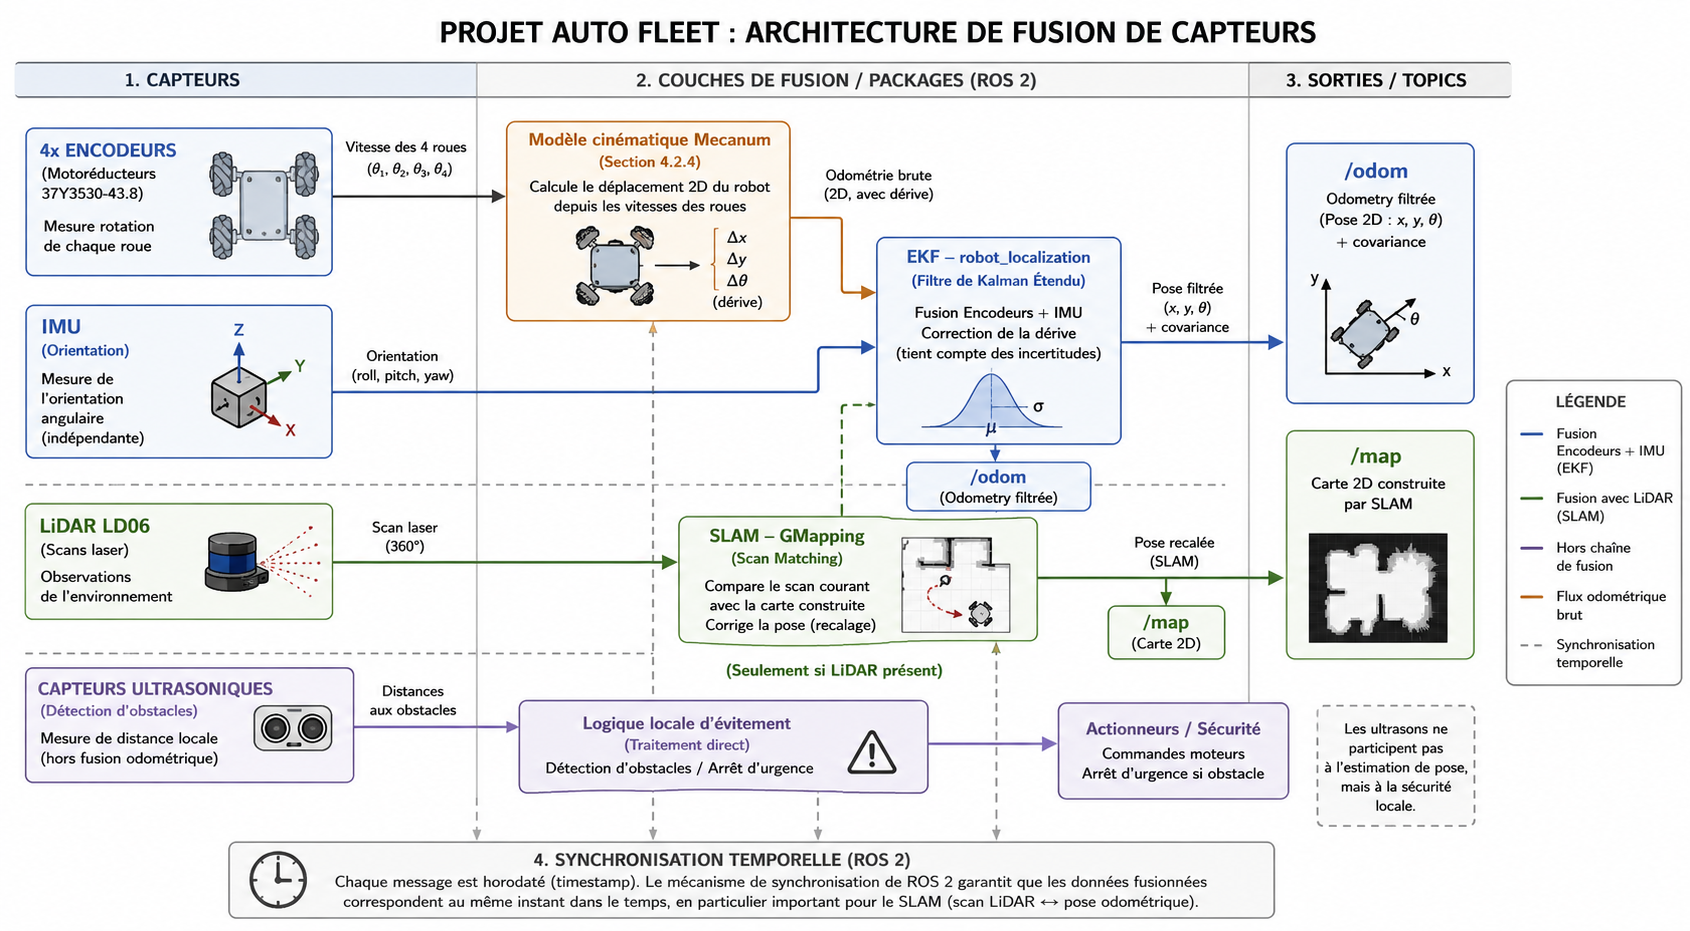
\includegraphics[width=0.9\textwidth]{images/perception_auto_fleet.png}
    \caption{Chaîne de perception et d’estimation d’état du projet Auto Fleet}
    \label{fig:perception_auto_fleet}
\end{figure}

\subsection{Cartographie partagée par SLAM}

Le \kw{SLAM} est l’un des pivots techniques du projet. Il permet de construire progressivement une carte tout en estimant la pose du robot dans cette même carte, sans a priori exhaustif sur l’environnement.

Dans Auto Fleet, cette fonction est assurée par \texttt{slam\_toolbox}. L’algorithme exploite les scans \kw{LiDAR} et l’odométrie enrichie pour corriger la trajectoire estimée, détecter des fermetures de boucle et mettre à jour la carte d’occupation.

Les robots de classe A produisent chacun une carte locale. Ces cartes sont ensuite fusionnées pour fournir une représentation plus large de la zone explorée. Cette carte partagée a plusieurs usages : soutien à la supervision, lecture de l’avancement de mission, et base potentielle de navigation pour d’autres unités.

Le \kw{SLAM} ne doit pas être lu uniquement comme un résultat cartographique. Il joue aussi un rôle de correction de pose. Une carte cohérente traduit généralement une chaîne perception--odométrie--recalage suffisamment stable ; une carte dégradée signale au contraire une faiblesse structurelle quelque part dans cette chaîne.

\subsection{Estimation d’état et prise de décision locale}

L’estimation d’état regroupe la pose du robot, sa vitesse, son orientation et une représentation simplifiée de son environnement immédiat. Cette estimation résulte de toute la chaîne de perception et constitue la base de la décision locale.

Sur les robots à roues mécanum, le modèle cinématique permet de passer des vitesses de roue au déplacement global du robot et réciproquement. Ce modèle alimente le calcul d’odométrie, mais il doit être interprété à la lumière des limites mécaniques réelles : une cinématique théoriquement correcte peut être dégradée par le glissement, les tolérances de montage ou les irrégularités du sol.

À partir de l’état estimé, le robot prend des décisions locales de navigation. La détection d’un obstacle proche, signalée par le \kw{LiDAR} ou les capteurs \kw{ultrasoniques}, conduit à une adaptation de trajectoire ou à un arrêt temporaire. Cette logique doit rester embarquée afin de préserver la réactivité du système, indépendamment de la latence de supervision.

Les informations d’état significatives sont enfin remontées vers la chaîne de supervision par l’intermédiaire du backend et du broker \outil{MQTT}. L’opérateur accède ainsi à une représentation synthétique de la situation de chaque robot sans intervenir dans les boucles de sécurité locales.

\section{Évaluation des performances de perception}

L’évaluation de la perception a pour fonction d’identifier ce qui est déjà exploitable et ce qui demeure insuffisamment robuste pour être considéré comme stabilisé.

\subsection{Détection d’obstacles et estimation de distance}

Les premiers essais ont porté sur la capacité des robots à détecter des obstacles et à en estimer la distance dans des conditions contrôlées.

Le \kw{LiDAR LD06} s’est montré particulièrement pertinent pour les obstacles situés dans son plan de balayage. Il fournit des mesures de distance compatibles avec les besoins de navigation et de cartographie, avec une résolution angulaire suffisante pour produire des contours exploitables par les algorithmes de recalage.

Les capteurs \kw{ultrasoniques} se sont révélés utiles à très courte distance, en particulier dans des configurations où le \kw{LiDAR} ne couvre pas exactement la zone la plus proche du châssis. Leur apport n’est pas de remplacer la perception géométrique fine, mais de compléter la sécurité locale.

Pour les robots sans \kw{LiDAR}, la détection rapide d’obstacles repose encore principalement sur les ultrasons, la caméra étant davantage mobilisée pour l’observation et l’exploration. Cette situation souligne un axe d’amélioration clair : l’exploitation plus poussée de la perception visuelle.

\subsection{Robustesse des mesures en environnement réel}

Les conditions réelles dégradent toujours, dans une certaine mesure, la qualité de la perception.

Les vibrations mécaniques générées par les roues mécanum ajoutent du bruit aux mesures \kw{IMU} et peuvent perturber le \kw{LiDAR} si le montage n’est pas suffisamment rigide. La qualité du sol joue également un rôle important, car elle conditionne l’adhérence et, par conséquent, la dérive des estimations fondées sur les encodeurs.

Les conditions d’éclairage influencent fortement la perception par \kw{caméra}. La version NoIR améliore la sensibilité en faible luminosité, mais ne supprime pas l’impact des contre-jours, des zones d’ombre ou des variations rapides d’exposition.

La présence d’objets mobiles complique enfin l’exploitation géométrique de l’environnement. Un \kw{SLAM} conçu pour un monde essentiellement statique peut être déstabilisé par des cibles en mouvement si aucun filtrage adapté n’est mis en œuvre. Ces difficultés ne remettent pas en cause la chaîne de perception ; elles définissent plutôt les limites de robustesse actuellement observables.

\subsection{Limites actuelles et pistes d’amélioration}

Plusieurs limites apparaissent déjà avec suffisamment de netteté pour orienter les développements futurs.

La première concerne la \kw{couverture spatiale} du \kw{LiDAR} 2D, limitée à un plan horizontal. Les obstacles hors plan ou les variations de niveau restent partiellement hors champ. Une amélioration possible consisterait à enrichir la perception verticale, soit par vision, soit par capteurs additionnels.

La deuxième limite touche à la \kw{dérive odométrique}, particulièrement sensible sur une base mécanum lorsque les déplacements latéraux deviennent fréquents. Même avec fusion capteurs, une erreur persistante peut s’accumuler. Des recalages externes plus riches ou des marqueurs visuels pourraient, à terme, réduire cette dépendance.

La troisième limite est liée à l’\kw{exploitation de la caméra}. Son potentiel reste largement supérieur à son usage actuel. Des développements de vision par ordinateur permettraient d’ajouter une dimension sémantique à la perception, absente d’une chaîne purement géométrique.

Enfin, la \kw{calibration extrinsèque} entre capteurs et la \kw{fusion des cartes multi-robots} constituent deux points où un formalisme plus poussé améliorerait sensiblement la qualité des résultats. Ces améliorations ne supposent pas nécessairement un changement de matériel ; elles demandent surtout une montée en maturité de la chaîne de traitement.

% =========================
% CHAPITRE 5
% =========================
\chapter{Communication entre robots et supervision (V2X)}
\label{chap:v2x}

La communication V2X constitue l'un des fondements du système \kw{Auto Fleet}. Elle assure la continuité des échanges entre les robots, la station de supervision et les services logiciels qui composent l'infrastructure de contrôle. Dans une flotte mobile, la qualité de ces échanges conditionne directement la réactivité des commandes, la cohérence de l'état affiché, la disponibilité des flux vidéo et la capacité du système à diagnostiquer une situation en cours de mission.

La solution retenue s'appuie sur une architecture distribuée : les fonctions de perception et d'action restent proches des robots, tandis que la supervision centralise l'observation, la coordination et la prise de décision opérateur. Cette séparation permet de conserver des robots autonomes au niveau local, tout en fournissant une vision globale de la flotte. Le système combine ainsi un robot embarqué sur \kw{Raspberry Pi}, un bus de messages \outil{MQTT}, un backend applicatif, une passerelle vidéo, une interface Web de supervision et des modules de perception capables d'intégrer caméra, Kinect, LiDAR et IMU.

\section{Objectifs de la couche V2X}

La couche V2X répond à trois objectifs principaux : transmettre les commandes avec un délai maîtrisé, maintenir une représentation fiable de l'état de la flotte et rendre les flux de perception exploitables par la supervision. Elle joue donc un rôle d'interface entre le monde robotique, fortement contraint par le temps réel et les capteurs, et le monde applicatif, orienté visualisation, diagnostic et interaction utilisateur.

\subsection{Contrat fonctionnel}

Le premier rôle de la couche V2X concerne la \kw{commande}. L'opérateur doit pouvoir sélectionner un robot, changer son mode, envoyer une consigne de téléopération, lancer une mission ou interrompre une action. Ces messages sont courts, mais leur priorité fonctionnelle est élevée. Le système associe chaque commande à un identifiant et à un retour d'exécution, ce qui permet de distinguer une commande reçue, appliquée ou rejetée.

Le deuxième rôle concerne la \kw{télémétrie}. Chaque robot publie périodiquement son état courant : mode, niveau de batterie, pose estimée, vitesse, état réseau, disponibilité des capteurs et horodatage. La supervision ne travaille pas directement sur des messages bruts ; elle consomme une représentation consolidée produite par le backend. Cette consolidation rend l'IHM indépendante du détail des protocoles et facilite l'ajout de nouveaux robots.

Le troisième rôle concerne les \kw{états de service}. Une flotte n'est pas uniquement composée de robots physiques ; elle dépend aussi de services logiciels tels que le broker de messages, le backend, la passerelle vidéo, les modules de perception et les agents embarqués. Le suivi de ces services permet de différencier une perte radio, une indisponibilité caméra, une interruption d'un flux vidéo ou une erreur applicative.

Le quatrième rôle concerne les \kw{flux de perception}. L'image couleur, la profondeur Kinect, les mesures LiDAR et les données IMU n'ont pas toutes la même fréquence, le même volume ou la même criticité. La couche V2X définit donc un format commun pour publier des états synthétiques : disponibilité du capteur, fréquence effective, qualité du signal, mesure minimale pertinente et niveau de confiance. Les données lourdes restent traitées par des modules spécialisés, tandis que la supervision reçoit une information directement exploitable.

\begin{table}[H]
\centering
\small
\renewcommand{\arraystretch}{1.18}
\begin{tabular}{|p{3.4cm}|p{3.0cm}|p{4.5cm}|p{4.0cm}|}
\hline
\textbf{Famille de données} & \textbf{Sens principal} & \textbf{Contenu} & \textbf{Rôle système} \\
\hline
Commandes & station vers robot & mode, téléopération, mission, arrêt & action opérateur et coordination \\
\hline
Télémétrie & robot vers station & batterie, pose, vitesse, état, horodatage & suivi temps réel de la flotte \\
\hline
Accusés de réception & robot vers station & identifiant, statut, délai, message & validation des commandes \\
\hline
États de service & services vers station & backend, broker, vidéo, perception, agent & diagnostic de l'infrastructure \\
\hline
Flux vidéo & robot vers passerelle, puis IHM & RTSP, MJPEG, snapshot & observation visuelle \\
\hline
Synthèse capteurs & robot vers station & caméra, Kinect, LiDAR, IMU, fusion & perception multi-capteurs \\
\hline
Alertes & robot ou backend vers station & obstacle, perte de lien, anomalie, mission & priorisation opérateur \\
\hline
\end{tabular}
\caption{Familles de données échangées dans la couche V2X}
\label{tab:v2x_messages_v2}
\end{table}

\subsection{Contraintes de communication}

Le système évolue sur un réseau local sans fil, donc dans un environnement où la latence, le jitter et la bande passante peuvent varier. L'architecture doit rester robuste lorsque la qualité radio fluctue, lorsque plusieurs flux vidéo sont actifs ou lorsque plusieurs robots publient simultanément leur télémétrie.

La \kw{latence} est critique pour la téléopération. Une commande doit atteindre le robot rapidement et produire un retour mesurable. Le système mesure donc le délai de bout en bout entre l'envoi d'un ordre et la réception de son accusé de réception. Cette mesure fournit une indication plus représentative de l'expérience opérateur qu'une simple latence réseau.

Le \kw{jitter} décrit la régularité des échanges. Dans une interface de supervision, des messages irréguliers peuvent produire des courbes instables et rendre difficile l'interprétation de l'état réel. Le backend maintient donc l'âge des derniers messages, la fréquence effective de réception et l'état de disponibilité de chaque robot.

La \kw{bande passante} concerne principalement la vidéo et les données de perception. Les messages MQTT restent légers, tandis que les flux visuels peuvent devenir coûteux. La passerelle vidéo applique des profils de qualité afin d'adapter la résolution et la compression au contexte d'utilisation. Les débits sont présentés en \kw{KB/s} et \kw{MB/s}, avec une base de calcul de 1024, afin de conserver une lecture homogène dans toute l'IHM.

\begin{table}[H]
\centering
\small
\renewcommand{\arraystretch}{1.18}
\begin{tabular}{|p{3.5cm}|p{5.6cm}|p{4.5cm}|}
\hline
\textbf{Indicateur} & \textbf{Interprétation} & \textbf{Utilisation} \\
\hline
Âge du heartbeat & temps écoulé depuis le dernier signe de vie & statut en ligne ou hors ligne \\
\hline
Latence télémétrie & délai estimé de remontée des données & fraîcheur des informations affichées \\
\hline
RTT commande & délai entre commande et accusé de réception & réactivité opérateur \\
\hline
Jitter & variabilité temporelle des messages & stabilité de la supervision \\
\hline
Débit & volume transféré en KB/s ou MB/s & choix du profil vidéo \\
\hline
Disponibilité vidéo & état du flux caméra et de la passerelle & distinction entre panne vidéo et panne robot \\
\hline
Qualité radio & indication de la robustesse du lien Wi-Fi & anticipation d'une dégradation \\
\hline
\end{tabular}
\caption{Indicateurs utilisés pour qualifier la communication V2X}
\label{tab:v2x_qos_v2}
\end{table}

\section{Architecture de communication}

L'architecture V2X repose sur une séparation nette entre trois niveaux : le niveau embarqué, le niveau applicatif et le niveau d'interface. Le niveau embarqué publie les données issues du robot et reçoit les commandes. Le niveau applicatif consolide les messages, applique les règles de supervision et expose une API stable. Le niveau d'interface présente les informations à l'opérateur et transmet ses décisions au backend.

\subsection{Rôle du backend}

Le backend constitue le point de convergence de la supervision. Il consomme les topics MQTT publiés par les robots et les services, maintient un état courant par robot et expose à l'IHM une structure homogène. Ce choix évite de faire dépendre le navigateur de la topologie MQTT et simplifie la logique d'affichage.

Le backend assure également la cohérence temporelle des données. Chaque message reçu est horodaté, associé à son robot et intégré dans une représentation consolidée. Cette représentation regroupe l'état robot, l'état réseau, les services actifs, la disponibilité vidéo et la synthèse capteurs. L'IHM peut ainsi afficher un état unique sans reconstituer elle-même les messages de bas niveau.

\subsection{Choix de MQTT et articulation avec ROS 2}

\outil{ROS 2} reste adapté aux échanges internes au robot : navigation, perception locale, contrôle et messages capteurs à forte fréquence. \outil{MQTT} est utilisé pour la couche de supervision, car il fournit un mécanisme léger de publication et d'abonnement, bien adapté à la télémétrie, aux états applicatifs et aux commandes de haut niveau.

Cette articulation évite de transformer l'IHM en client direct du middleware robotique. Les robots conservent leur logique embarquée, tandis que la station de supervision reçoit des messages normalisés. L'ajout d'un nouveau robot consiste à publier les mêmes familles de topics avec un nouvel identifiant, sans modifier la structure générale de la supervision.

\begin{table}[H]
\centering
\small
\renewcommand{\arraystretch}{1.18}
\begin{tabular}{|p{4.4cm}|p{4.4cm}|p{5.2cm}|}
\hline
\textbf{Topic logique} & \textbf{Producteur principal} & \textbf{Utilisation} \\
\hline
\texttt{fleet/v1/telemetry/R1} & agent robot & état courant et données réseau \\
\hline
\texttt{fleet/v1/heartbeat/R1} & agent robot & présence et disponibilité \\
\hline
\texttt{fleet/v1/command/R1} & backend & commande de mode, mission ou téléopération \\
\hline
\texttt{fleet/v1/ack/R1} & agent robot & retour sur commande \\
\hline
\texttt{fleet/v1/video\_status/R1} & passerelle vidéo & état du flux, résolution, FPS, débit \\
\hline
\texttt{fleet/v1/sensor/R1} & agent robot & synthèse caméra, Kinect, LiDAR, IMU \\
\hline
\texttt{fleet/v1/heartbeat/backend} & backend & disponibilité de la supervision \\
\hline
\end{tabular}
\caption{Organisation des topics de supervision}
\label{tab:v2x_topics}
\end{table}

\subsection{Découverte et adaptation au réseau}

La supervision intègre une logique de découverte réseau afin de rester exploitable lorsque l'environnement change. Les robots et les services sont identifiés par leur rôle, leur disponibilité et les ports applicatifs qu'ils exposent. La station peut ainsi vérifier la présence d'un robot, qualifier l'accessibilité de ses flux et mettre à jour les endpoints utilisés par la supervision.

Cette capacité est importante pour une flotte mobile, car l'adresse d'un robot peut évoluer selon le réseau utilisé. La découverte ne remplace pas la configuration nominale, mais elle réduit la dépendance à des adresses figées et accélère le retour en service. Elle participe également au diagnostic, en distinguant un robot absent, un service indisponible et un flux vidéo non joignable.

\begin{figure}[H]
    \centering
    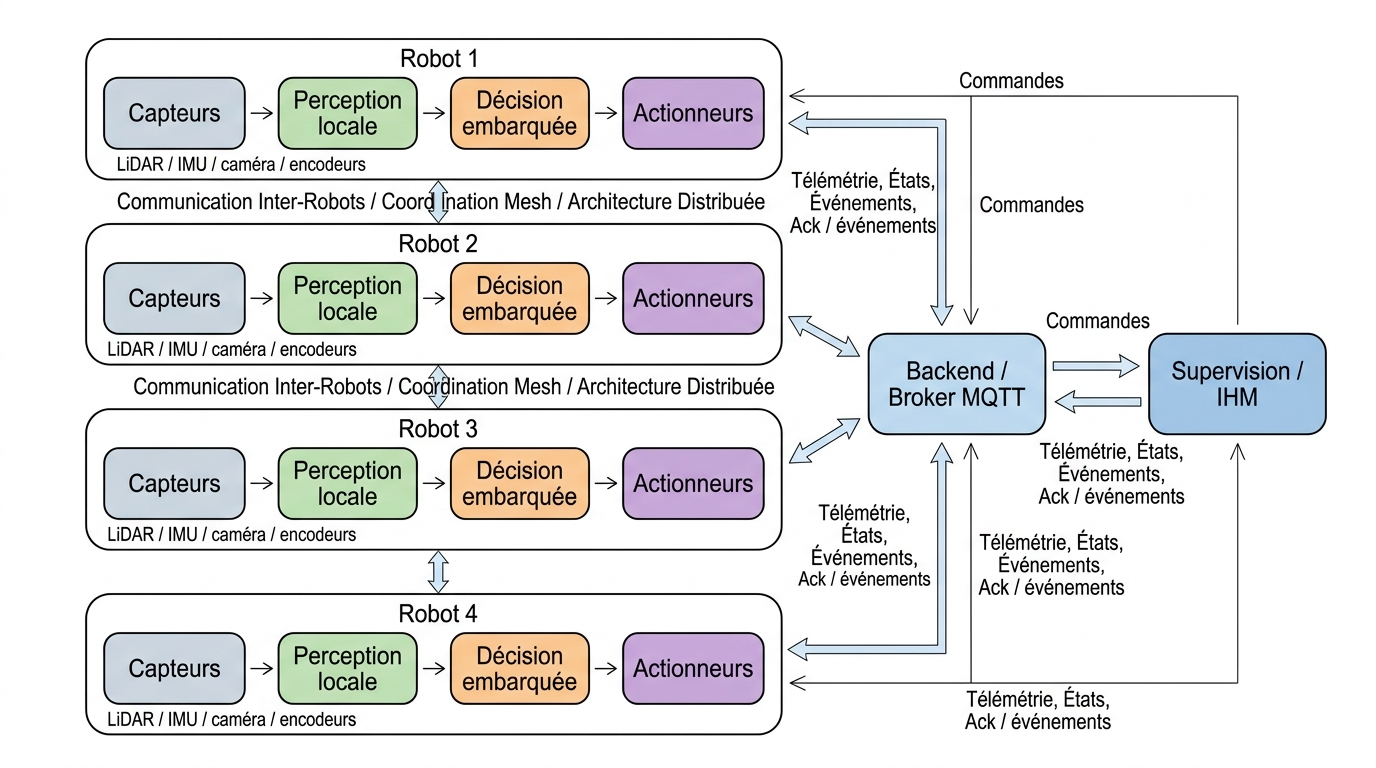
\includegraphics[width=0.92\textwidth]{images/archi_generale_v2.png}
    \caption{Architecture logique de la communication V2X}
    \label{fig:v2x_architecture_logicielle_v2}
\end{figure}

\section{Supervision Web et interaction opérateur}

L'IHM fournit une vue unifiée de la flotte et des services qui la supportent. Elle regroupe le suivi des robots, la téléopération, les commandes de mission, les courbes réseau, l'état vidéo, les alertes et les informations de perception. Son rôle est de rendre la situation exploitable par l'opérateur, sans exposer directement la complexité des flux internes.

\subsection{Vue flotte}

La vue flotte présente chaque robot sous forme de ligne synthétique. Elle affiche l'identifiant, l'état en ligne, le mode courant, la batterie, l'âge du dernier message, la latence, le jitter, le débit, le RTT de commande, la disponibilité vidéo et l'état des capteurs principaux.

Cette approche permet de comparer rapidement plusieurs robots et d'identifier les priorités d'intervention. Un robot peut être disponible pour les commandes mais privé de vidéo ; un autre peut conserver son flux visuel tout en présentant une télémétrie dégradée. La séparation des indicateurs rend ces cas lisibles.

\subsection{Commandes et accusés de réception}

Les commandes opérateur transitent par le backend avant d'être publiées vers le robot cible. Le backend attribue un identifiant à chaque ordre, conserve le contexte d'envoi et attend le retour associé. Le robot publie ensuite un accusé de réception décrivant l'état de la commande.

Ce mécanisme apporte deux garanties. Il permet d'abord à l'IHM d'afficher un retour explicite à l'opérateur. Il permet ensuite de mesurer le temps de réponse réel du robot, en incluant le trajet applicatif complet. Cette mesure sert à qualifier la réactivité de la flotte pendant une mission.

\subsection{Vidéo et profils de qualité}

La vidéo est traitée par une passerelle dédiée. Le robot publie un flux RTSP, puis la passerelle le convertit en MJPEG pour l'affichage Web. Ce choix assure une intégration simple dans le navigateur et maintient la conversion vidéo dans un service isolé, plus facile à surveiller et à adapter.

Quatre profils de qualité sont disponibles. Ils agissent sur la largeur maximale, la qualité JPEG et l'intervalle d'envoi MJPEG. Le profil le plus réactif réduit la résolution afin de minimiser la latence perçue, tandis que les profils de qualité supérieure améliorent la lisibilité lorsque le réseau et la charge processeur le permettent.

\begin{table}[H]
\centering
\small
\renewcommand{\arraystretch}{1.18}
\begin{tabular}{|p{3.2cm}|p{2.3cm}|p{2.5cm}|p{2.8cm}|p{3.6cm}|}
\hline
\textbf{Profil} & \textbf{Largeur max.} & \textbf{Qualité JPEG} & \textbf{Intervalle MJPEG} & \textbf{Usage visé} \\
\hline
Ultra Low Latency & 360 px & 54 & 40 ms & priorité à la réactivité \\
\hline
Balanced & 640 px & 68 & 30 ms & compromis par défaut \\
\hline
Quality & 960 px & 76 & 35 ms & meilleure lisibilité visuelle \\
\hline
High Quality & 1280 px & 82 & 45 ms & observation détaillée \\
\hline
\end{tabular}
\caption{Profils de qualité disponibles pour la vidéo}
\label{tab:v2x_video_profiles}
\end{table}

\subsection{Diagnostic réseau}

Le diagnostic réseau rassemble les mesures de latence, jitter, RTT, perte et débit. Les valeurs de débit sont affichées de manière homogène en KB/s ou MB/s. Cette présentation correspond à la lecture attendue par l'opérateur pour des volumes de données, notamment les flux vidéo.

La supervision peut également estimer la charge induite par plusieurs flux simultanés. Cette estimation aide à déterminer si la priorité doit être donnée à la qualité visuelle ou à la réactivité. Elle prépare aussi le passage à une flotte plus grande, où l'affichage de toutes les vidéos en haute qualité ne constitue pas toujours le meilleur choix opérationnel.

\begin{figure}[H]
    \centering
    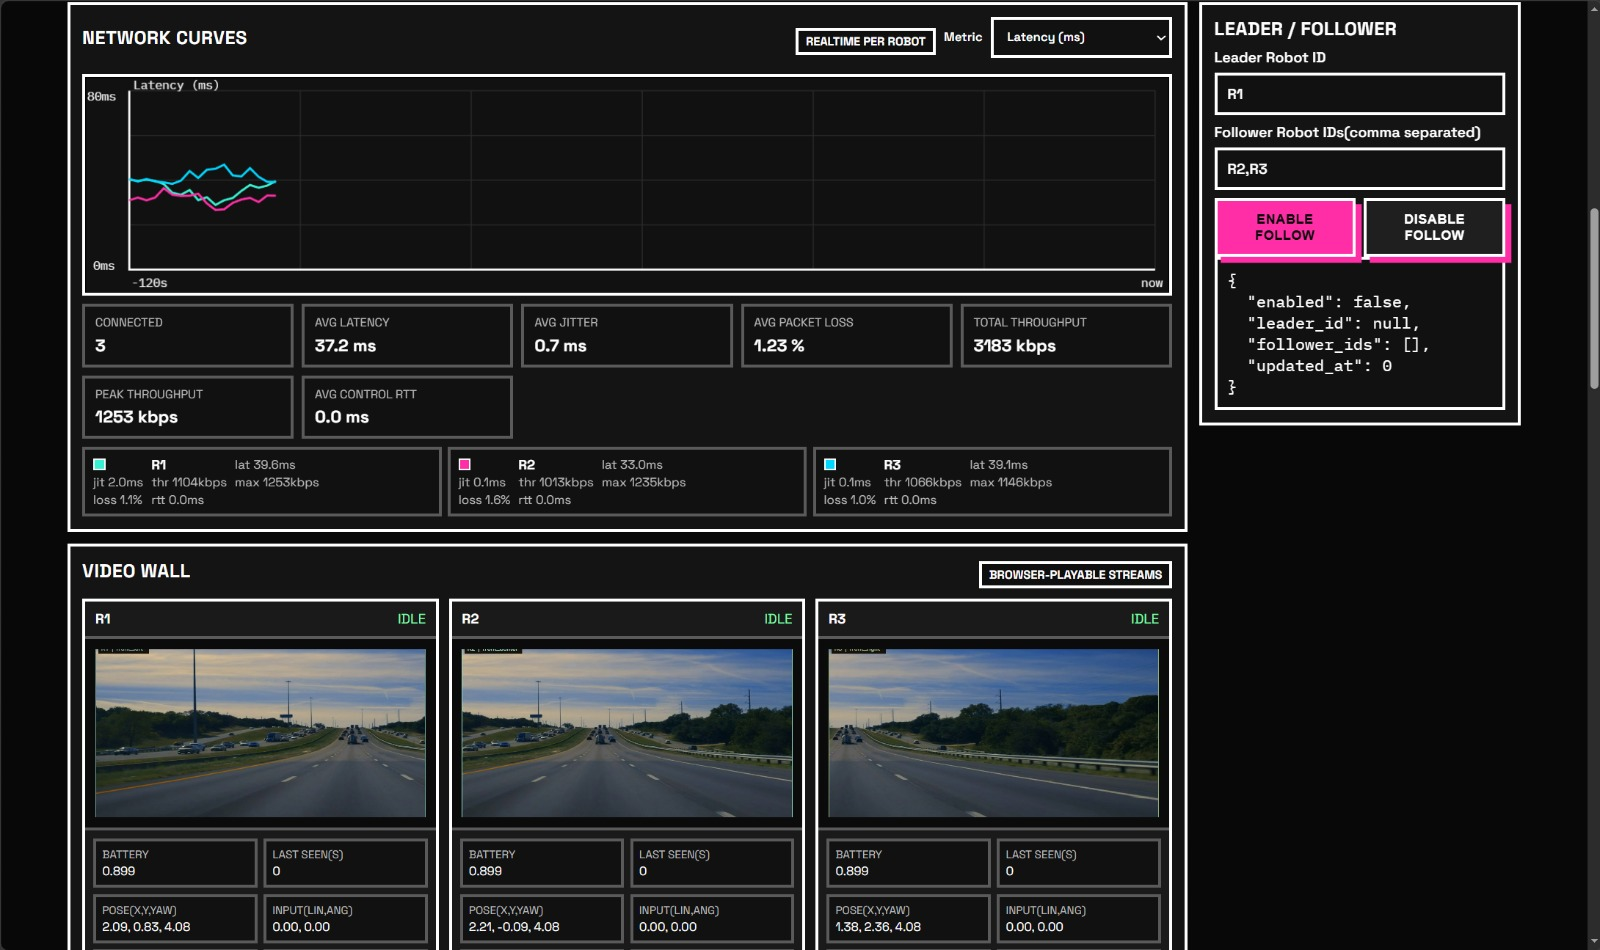
\includegraphics[width=0.92\textwidth]{images/baba.png}
    \caption{Organisation générale de l'IHM de supervision}
    \label{fig:v2x_ihm_generale_v2}
\end{figure}

\section{Intégration robot et perception multi-capteurs}

Le robot R1 représente l'implémentation complète de la chaine V2X sur une plateforme réelle. Il associe un agent embarqué, une caméra, un flux vidéo, une télémétrie MQTT et des états capteurs publiés vers la supervision. Cette intégration valide le passage d'une architecture logicielle à une chaine robotique observable et commandable.

\subsection{Agent embarqué}

L'agent embarqué joue le rôle d'adaptateur entre le robot et la supervision. Il publie la télémétrie, les heartbeats, les accusés de réception et la synthèse capteurs. Il reçoit les commandes de haut niveau et les transmet aux fonctions locales du robot.

Cette séparation permet de garder une frontière claire entre la logique embarquée et la supervision. Les traitements bas niveau restent du côté robot, tandis que la station reçoit des états normalisés. La même structure peut être reproduite sur d'autres robots de la flotte.

\begin{table}[H]
\centering
\small
\renewcommand{\arraystretch}{1.18}
\begin{tabular}{|p{4.0cm}|p{6.0cm}|p{3.6cm}|}
\hline
\textbf{Élément} & \textbf{Fonction} & \textbf{Rôle V2X} \\
\hline
Agent robot & publication MQTT et réception des commandes & interface embarquée \\
\hline
Caméra RGB & acquisition visuelle et flux RTSP & observation vidéo \\
\hline
Kinect & profondeur et estimation de distance & perception 3D \\
\hline
LiDAR & distances et obstacles & navigation et sécurité \\
\hline
IMU & orientation et mouvements & stabilisation et diagnostic \\
\hline
Backend & agrégation des messages & état consolidé \\
\hline
IHM & affichage et interaction & supervision opérateur \\
\hline
\end{tabular}
\caption{Rôle des composants dans l'intégration V2X de R1}
\label{tab:v2x_r1_integration}
\end{table}

\subsection{Chaîne vidéo}

La chaîne vidéo relie l'acquisition embarquée à l'affichage Web. La caméra produit un flux sur le robot, ce flux est publié en RTSP, puis converti par la passerelle en MJPEG. La supervision reçoit en parallèle l'état du flux : disponibilité, résolution, fréquence, débit et URL de snapshot.

Ce découpage isole les responsabilités. Le robot se concentre sur l'acquisition et la publication du flux. La passerelle gère la conversion et les profils de qualité. Le navigateur affiche un format simple, compatible et léger à intégrer. Cette organisation limite le couplage entre matériel caméra, protocole vidéo et interface utilisateur.

\subsection{Synthèse capteurs}

La supervision ne se limite pas à l'image RGB. La Kinect fournit une information de profondeur exploitable pour estimer les distances et enrichir l'analyse de l'environnement. Le LiDAR apporte une mesure de distance plus adaptée à la détection d'obstacles et à la cartographie. L'IMU complète ces informations par l'orientation, les accélérations et la détection de mouvements brusques.

Les données capteurs sont ramenées à une synthèse commune avant affichage. Pour chaque capteur, le message indique l'état, la fréquence, la dernière mise à jour, la mesure principale et un niveau de confiance. Cette approche évite de saturer l'IHM avec des données brutes et fournit à l'opérateur des informations directement interprétables.

\begin{figure}[H]
    \centering
    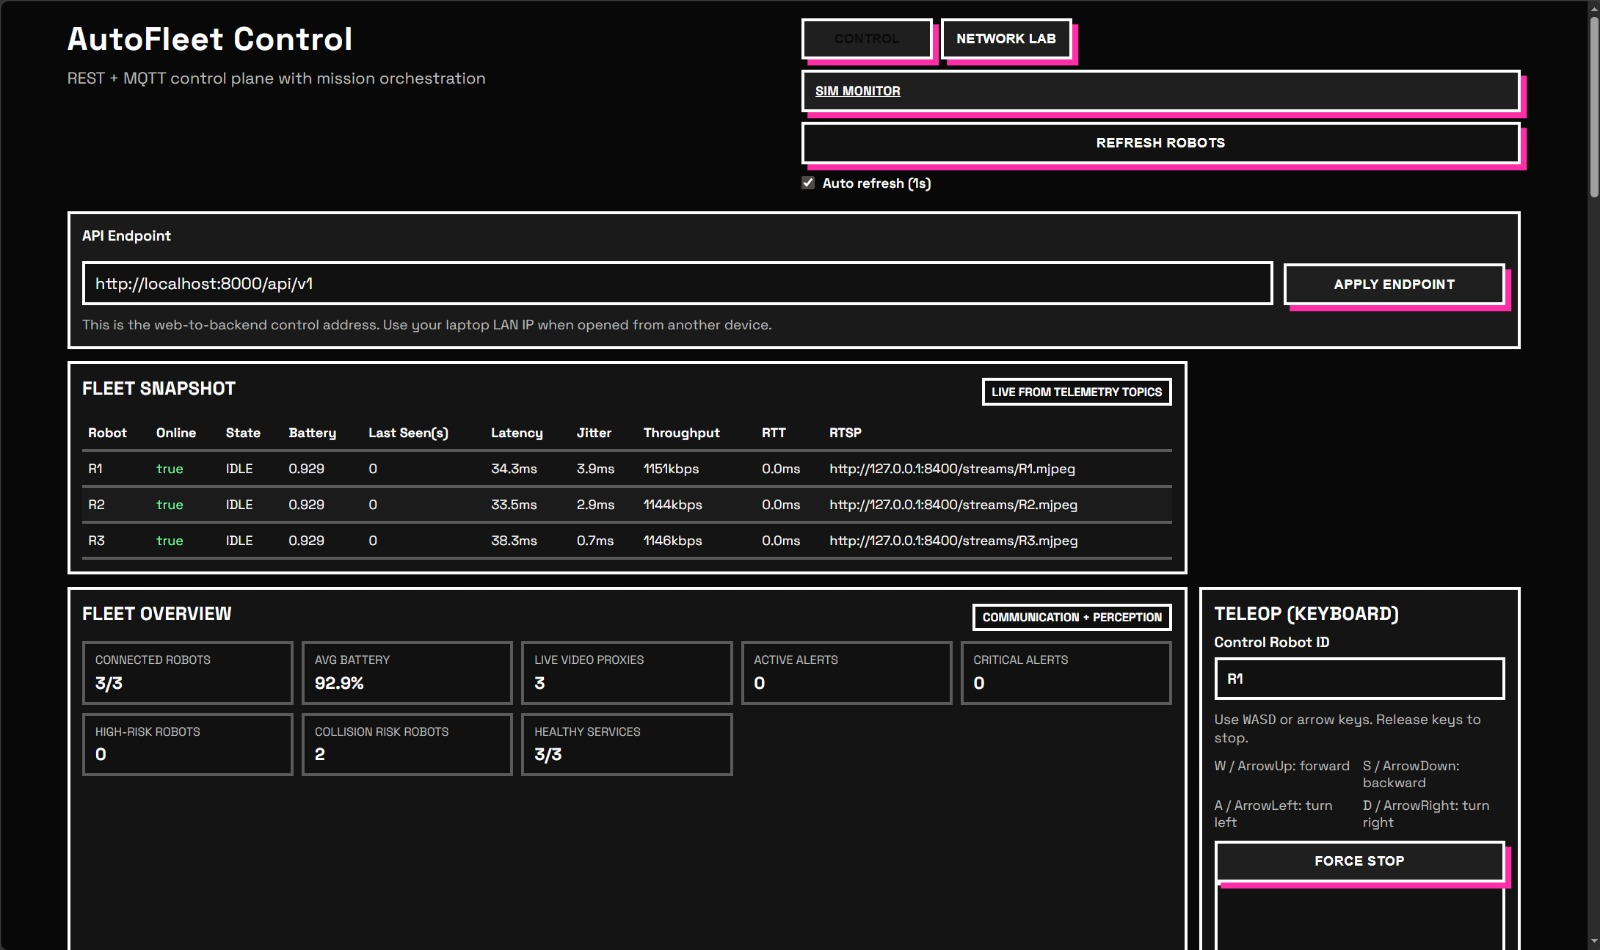
\includegraphics[width=0.92\textwidth]{images/7.jpg}
    \caption{Vue de diagnostic réseau et de gestion des flux vidéo}
    \label{fig:v2x_diagnostic_reseau_v2}
\end{figure}

\section{Validation de l'architecture}

La validation de la couche V2X s'appuie sur la cohérence entre les messages publiés, l'état consolidé côté backend et l'affichage dans l'IHM. Le système est validé lorsque les commandes, la télémétrie, la vidéo, les états de service et la synthèse capteurs restent cohérents dans la supervision.

\subsection{Résultats obtenus}

La chaine réalisée permet à la station de recevoir la télémétrie de R1, d'envoyer des commandes, de mesurer les délais de réponse, d'afficher le flux vidéo et de présenter l'état des capteurs. Les indicateurs réseau sont visibles dans l'IHM, les débits sont exprimés en KB/s ou MB/s et les profils vidéo peuvent être appliqués à l'ensemble des robots affichés.

Ces résultats valident l'architecture retenue : le backend joue son rôle de couche de consolidation, MQTT fournit un transport léger pour la supervision, la passerelle vidéo rend le flux exploitable par le navigateur et l'IHM présente une lecture unifiée de la flotte.

\subsection{Scalabilité}

L'architecture est conçue pour évoluer vers plusieurs robots. Les topics utilisent un identifiant robot, les états sont maintenus par entité et les profils vidéo s'appliquent de manière homogène. L'ajout d'un robot revient donc à ajouter une nouvelle instance de publication respectant le même contrat de messages.

La supervision peut ensuite hiérarchiser l'affichage selon le nombre de robots : vue synthétique pour la flotte, détails à la demande, priorisation des alertes et adaptation des flux vidéo. Cette logique évite que l'augmentation du nombre de robots se traduise par une surcharge directe de l'interface.

\subsection{Perspectives d'évolution}

Les évolutions principales concernent l'adaptation dynamique. Le système peut ajuster automatiquement le profil vidéo selon la latence, le débit disponible et la charge CPU. Les informations Kinect, LiDAR et IMU peuvent également être fusionnées pour produire une perception plus riche : distance minimale, obstacle prioritaire, orientation, stabilité et confiance globale.

Une évolution vers WebRTC peut être envisagée pour les scénarios où la latence vidéo devient prioritaire. Cette évolution ne modifie pas le principe d'architecture : le robot publie un flux, une passerelle spécialisée l'adapte et l'IHM consomme une représentation compatible avec le Web.

\begin{table}[H]
\centering
\small
\renewcommand{\arraystretch}{1.18}
\begin{tabular}{|p{3.4cm}|p{5.4cm}|p{5.0cm}|}
\hline
\textbf{Axe} & \textbf{Réalisation} & \textbf{Évolution} \\
\hline
Réseau & découverte, heartbeat, mesure RTT & sélection automatique du meilleur chemin \\
\hline
Vidéo & RTSP vers MJPEG, profils qualité & adaptation dynamique et WebRTC \\
\hline
Capteurs & caméra, Kinect, LiDAR, IMU & fusion multi-capteurs \\
\hline
Supervision & vue flotte, commandes, diagnostic & priorisation et historique enrichi \\
\hline
Scalabilité & topics par robot, état consolidé & orchestration multi-robots avancée \\
\hline
\end{tabular}
\caption{Synthèse de la validation et des évolutions V2X}
\label{tab:v2x_perspectives}
\end{table}

En conclusion, la couche V2X fournit l'infrastructure de communication nécessaire à une flotte supervisée. Elle relie les robots, les services applicatifs, les flux vidéo et les capteurs dans une architecture cohérente. Cette base permet d'assurer la commande, l'observation, le diagnostic et l'extension multi-capteurs du système \kw{Auto Fleet}.


\iffalse
\chapter{Communication entre robots et supervision (V2X)}

La communication n’est pas traitée dans Auto Fleet comme une couche auxiliaire. Elle est l’un des mécanismes qui rendent la flotte observable, coordonnable et exploitable depuis une station de supervision sans annuler l’autonomie locale des robots.

\section{Enjeux de communication et de supervision de la flotte}

L’architecture de communication doit permettre à la fois le transport des ordres, la remontée des états et la lecture globale de la mission. Elle doit aussi accepter une qualité réseau imparfaite sans faire dépendre entièrement la sécurité du système d’un lien sans faille.

\subsection{Besoins d’échange entre robots et station}

Les échanges entre robots et station couvrent plusieurs familles fonctionnelles.

La première concerne les \kw{commandes}. L’opérateur doit pouvoir lancer une mission, changer de mode, interrompre une action, sélectionner un robot ou transmettre une consigne de déplacement dans le cadre d’un contrôle manuel.

La deuxième correspond aux \kw{états robots}. Disponibilité, niveau de batterie, mode courant, erreurs et état global du système doivent être remontés régulièrement afin que la station dispose d’une vision consolidée de la flotte.

La troisième famille regroupe la \kw{télémétrie} : pose estimée, vitesse, orientation, indicateurs capteurs et informations de mission. Ces données fournissent à l’opérateur un retour continu sur le comportement des robots.

Une quatrième catégorie concerne les \kw{événements} : apparition d’un obstacle bloquant, perte de liaison, validation d’une action, alarme ou fin d’étape. Ces messages sont moins fréquents, mais plus structurants pour l’interprétation de la mission.

Enfin, pour les robots équipés d’un \kw{LiDAR}, certaines données participent à la \kw{cartographie partagée}. Leur importance tient moins à leur fréquence qu’à leur rôle dans la construction d’une représentation globale de l’environnement.

Le \kw{Tableau~\ref{tab:v2x_messages}} récapitule ces familles d’échanges.

\begin{table}[H]
\centering
\small
\renewcommand{\arraystretch}{1.15}
\begin{tabular}{|p{3.4cm}|p{2.5cm}|p{4.2cm}|p{4.2cm}|}
\hline
\textbf{Catégorie} & \textbf{Sens} & \textbf{Contenu principal} & \textbf{Utilité} \\
\hline
Commandes & station vers robots & ordre de déplacement, changement de mode, lancement ou arrêt de mission & contrôle opérateur \\
\hline
États robots & robots vers station & disponibilité, batterie, mode courant, erreurs & supervision globale \\
\hline
Télémétrie & robots vers station & position, vitesse, orientation, horodatage & suivi temps réel \\
\hline
Événements & robots vers station & obstacle, alarme, mission atteinte, perte de liaison & compréhension du contexte \\
\hline
Données de carte & robots LiDAR vers backend & informations utiles au SLAM partagé & cartographie de la zone \\
\hline
Références vidéo & backend vers IHM & disponibilité et accès aux flux & observation visuelle \\
\hline
\end{tabular}
\caption{Principales familles d’échanges dans la chaîne V2X}
\label{tab:v2x_messages}
\end{table}

\subsection{Contraintes réseau du système}

La communication s’inscrit dans un environnement réseau nécessairement imparfait. Les robots se déplacent, la charge réseau varie et la stabilité radio n’est jamais totalement garantie.

La \kw{latence} constitue une première contrainte forte. Une supervision utile suppose que les retours ne soient pas trop éloignés des événements réels. Le \kw{jitter} joue un rôle complémentaire : même avec une latence moyenne acceptable, une trop grande variabilité temporelle rend l’affichage irrégulier et dégrade la lisibilité de l’interface.

La \kw{perte de messages} doit également être considérée en fonction de la criticité des flux. Une perte ponctuelle sur une télémétrie régulière n’a pas la même gravité qu’une perte sur une commande ou sur un accusé de réception critique. Il faut donc penser l’architecture non seulement en termes de volume de données, mais aussi en termes de \kw{priorité fonctionnelle}.

La \kw{bande passante} disponible n’est pas illimitée. Les messages de contrôle restent généralement légers, mais les flux vidéo et certaines données de cartographie peuvent rapidement saturer un lien si aucune hiérarchisation n’est prévue.

Le \kw{Tableau~\ref{tab:v2x_qos}} résume les indicateurs réseau surveillés dans le cadre du projet.

\begin{table}[H]
\centering
\small
\renewcommand{\arraystretch}{1.15}
\begin{tabular}{|p{4.1cm}|p{5.2cm}|p{4.0cm}|}
\hline
\textbf{Indicateur} & \textbf{Rôle dans le projet} & \textbf{Effet d’une dérive} \\
\hline
Latence & temps de traversée des échanges & supervision moins réactive \\
\hline
Jitter & régularité temporelle des messages & affichage instable \\
\hline
Perte de messages & fiabilité des échanges & informations manquantes \\
\hline
Débit & capacité à porter plusieurs flux & saturation de l’IHM ou du lien \\
\hline
RSSI & qualité radio perçue & déconnexion ou baisse de portée \\
\hline
RTT commande & réactivité perçue par l’opérateur & retard de prise en compte \\
\hline
\end{tabular}
\caption{Principales contraintes réseau observées dans la supervision}
\label{tab:v2x_qos}
\end{table}

\subsection{Place de la supervision dans l’architecture globale}

La supervision se situe au-dessus de la logique embarquée. Elle n’assure ni les boucles de sécurité immédiates ni les réactions de proximité ; elle fournit une \kw{lecture consolidée} de la flotte et des moyens d’action coordonnés.

Dans l’architecture Auto Fleet, la station de supervision dialogue avec un \kw{backend} qui agrège les informations, prépare les messages, reçoit les télémétries et met en forme les données destinées à l’interface. Ce backend évite d’exposer directement l’IHM aux détails de communication de chaque robot.

La supervision n’est donc ni un simple tableau de bord, ni un poste de téléopération au sens strict. Elle constitue une couche intermédiaire entre \kw{visibilité}, \kw{diagnostic}, \kw{pilotage de haut niveau} et \kw{suivi de mission}.

\begin{figure}[H]
    \centering
    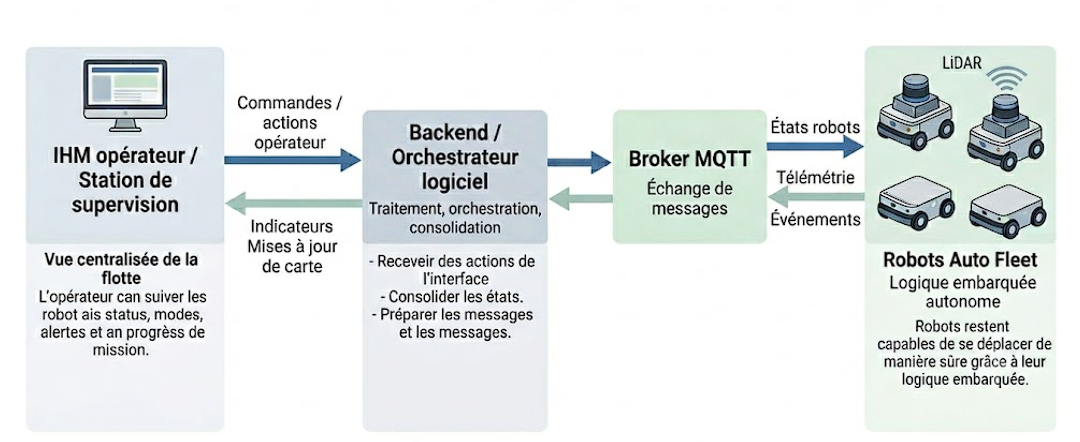
\includegraphics[width=0.92\textwidth]{images/Papa.png}
    \caption{Position de la supervision dans l’architecture globale}
    \label{fig:v2x_supervision_place}
\end{figure}

\section{Mise en œuvre de l’architecture V2X et de l’IHM}

La chaîne V2X retenue repose sur une séparation explicite entre interface utilisateur, backend applicatif, broker de messages et robots. Ce découpage vise à contenir la complexité et à rendre les responsabilités plus lisibles.

\subsection{Architecture logicielle de communication}

L’IHM constitue la couche visible pour l’opérateur. Les actions déclenchées côté interface sont transmises au backend, qui les traduit et les diffuse vers les robots au moyen du broker \outil{MQTT}. Les robots publient en retour leurs états, leur télémétrie, leurs événements et leurs accusés de réception.

Le broker joue ici un rôle d’\kw{intermédiaire asynchrone}. Il limite le couplage direct entre les producteurs et les consommateurs de messages, ce qui facilite l’ajout, le retrait ou la reconfiguration d’un robot sans redéfinir toute la chaîne applicative.

Le backend ne se contente pas de relayer. Il \kw{consolide} les informations, produit une vue cohérente de l’état global de la flotte et expose à l’IHM des structures plus simples à afficher. Cette couche intermédiaire permet de distinguer les contraintes de communication bas niveau des besoins de lisibilité de la supervision.

Le recours à \outil{MQTT} pour la supervision ne contredit pas l’usage de \outil{ROS 2} à l’intérieur des robots. Les deux se complètent : \outil{ROS 2} structure les flux techniques internes, tandis que \outil{MQTT} offre une couche adaptée au backend, à la supervision et à la dissociation des producteurs de données.

\begin{figure}[H]
    \centering
    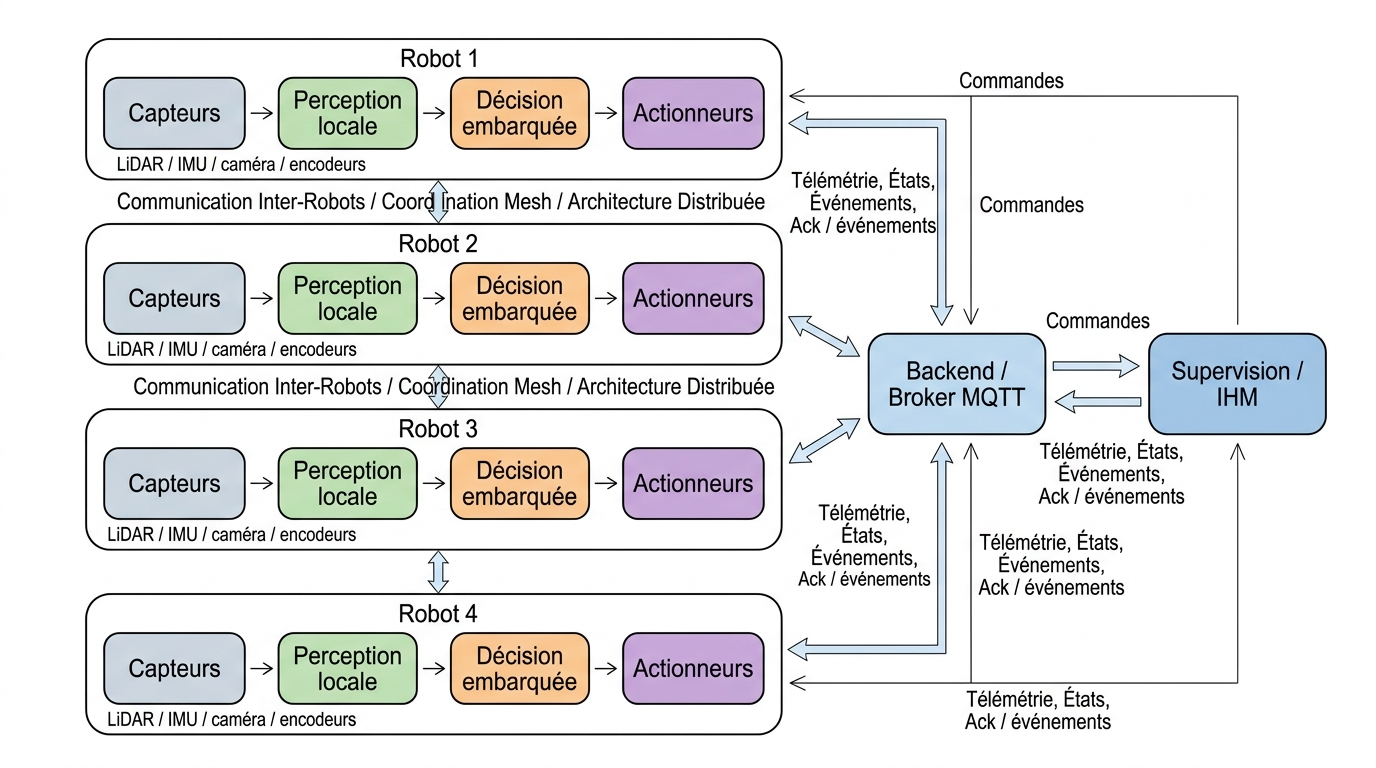
\includegraphics[width=0.92\textwidth]{images/archi_generale_v2.png}
    \caption{Architecture logicielle complète de la communication V2X}
    \label{fig:v2x_architecture_logicielle}
\end{figure}

\subsection{Interface de supervision et de contrôle}

L’interface de supervision doit rendre lisible un système potentiellement chargé en données. L’enjeu n’est pas d’afficher le maximum d’informations, mais d’exposer celles qui permettent une compréhension rapide de l’état courant de la flotte.

L’IHM regroupe plusieurs fonctions. Une première fonction concerne le \kw{contrôle} : sélection d’un robot, émission d’une commande, changement de mode, lancement ou interruption d’une mission. Une deuxième fonction relève du \kw{suivi d’état} : disponibilité des robots, connexion, batterie, états synthétiques et alertes.

Une troisième fonction regroupe la \kw{visualisation des retours}. L’interface doit permettre de consulter la télémétrie, les événements, certains indicateurs réseau et, lorsque le système est stabilisé, les informations utiles à la cartographie ou à la vidéo.

Le besoin de supervision est d’autant plus marqué que la flotte n’est pas homogène. L’IHM doit permettre d’identifier rapidement quels robots produisent des cartes, lesquels ne disposent que d’une perception visuelle, lesquels sont momentanément dégradés, et quels éléments de mission sont bloquants.

\begin{figure}[H]
    \centering
    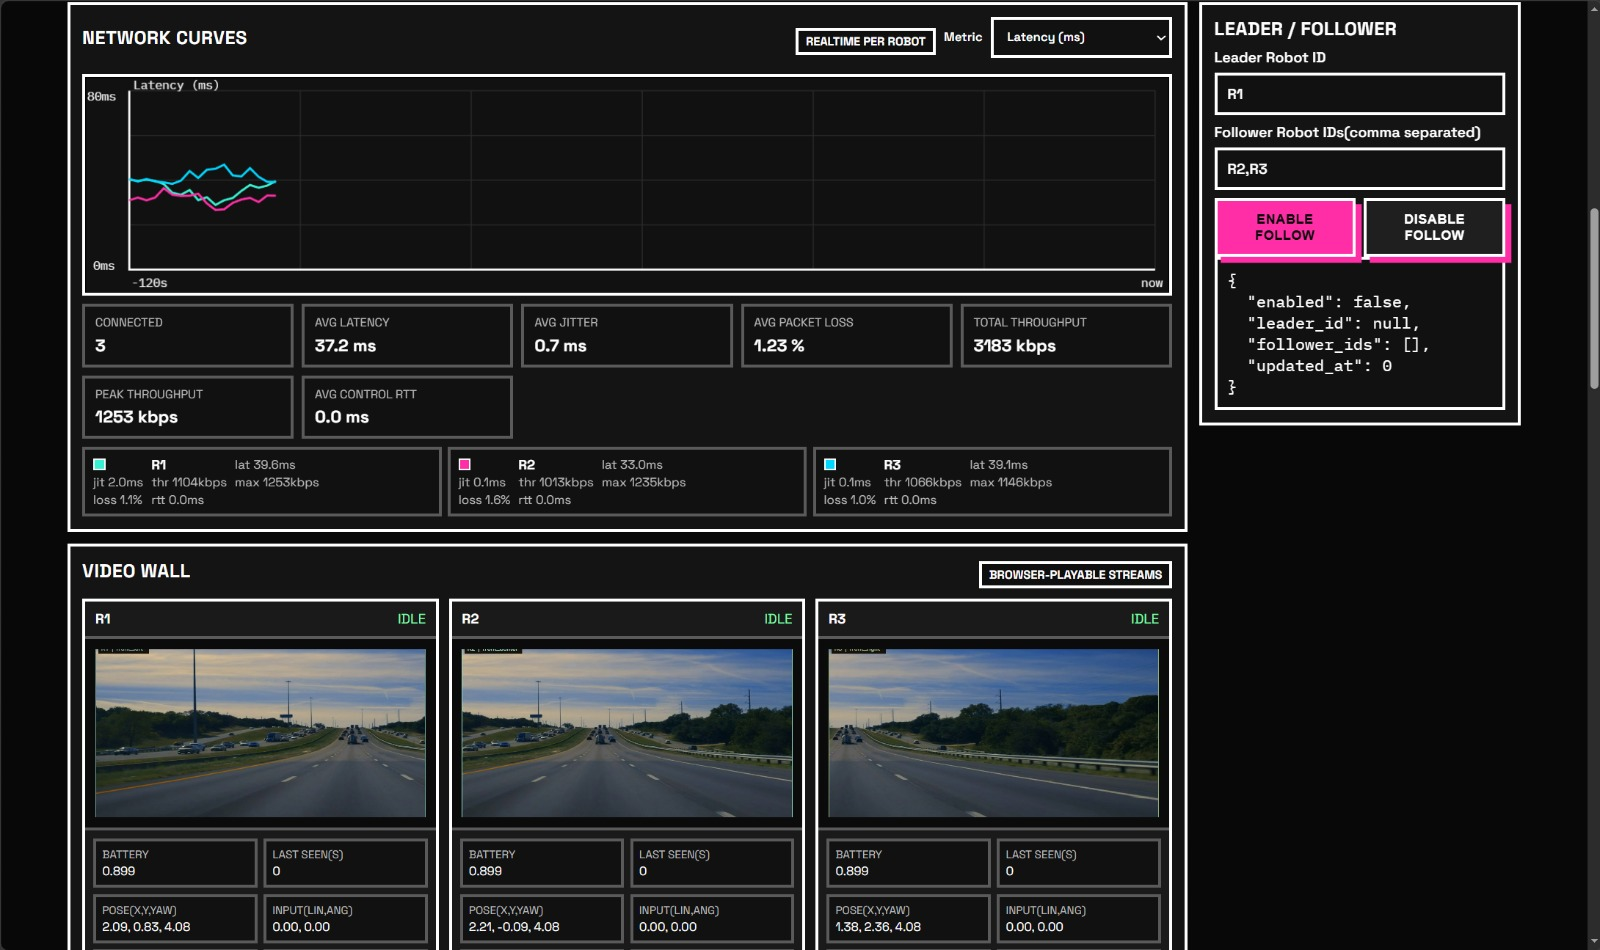
\includegraphics[width=0.92\textwidth]{images/baba.png}
    \caption{Organisation générale de l’IHM de supervision}
    \label{fig:v2x_ihm_generale}
\end{figure}

\subsection{Gestion des flux vidéo et diagnostic réseau}

Les flux vidéo occupent une place particulière dans l’architecture. Ils ne sont pas indispensables à la logique minimale de supervision, mais ils enrichissent fortement l’interprétation d’une situation locale, notamment lors de blocages, de détections ambiguës ou de démonstrations.

Dans Auto Fleet, les flux sont considérés comme des apports complémentaires à la télémétrie. Le backend peut référencer des flux \kw{RTSP} et exposer à l’IHM leur disponibilité sans nécessairement retraiter lui-même l’intégralité de la vidéo.

Cette décision s’accompagne d’une vigilance particulière sur la charge réseau. La vidéo est coûteuse et peut, si elle n’est pas maîtrisée, affecter la fluidité des autres échanges. C’est pourquoi le diagnostic réseau n’est pas accessoire : il permet de savoir si l’infrastructure supporte simultanément la télémétrie, les commandes, les retours de mission et les flux lourds.

Le diagnostic rassemble ainsi plusieurs mesures : \kw{latence}, \kw{jitter}, \kw{RTT}, \kw{perte de messages}, \kw{débit} et \kw{RSSI}. Ces indicateurs donnent une lecture plus précise du comportement réel du système que la simple observation visuelle de l’IHM.

\begin{figure}[H]
    \centering
    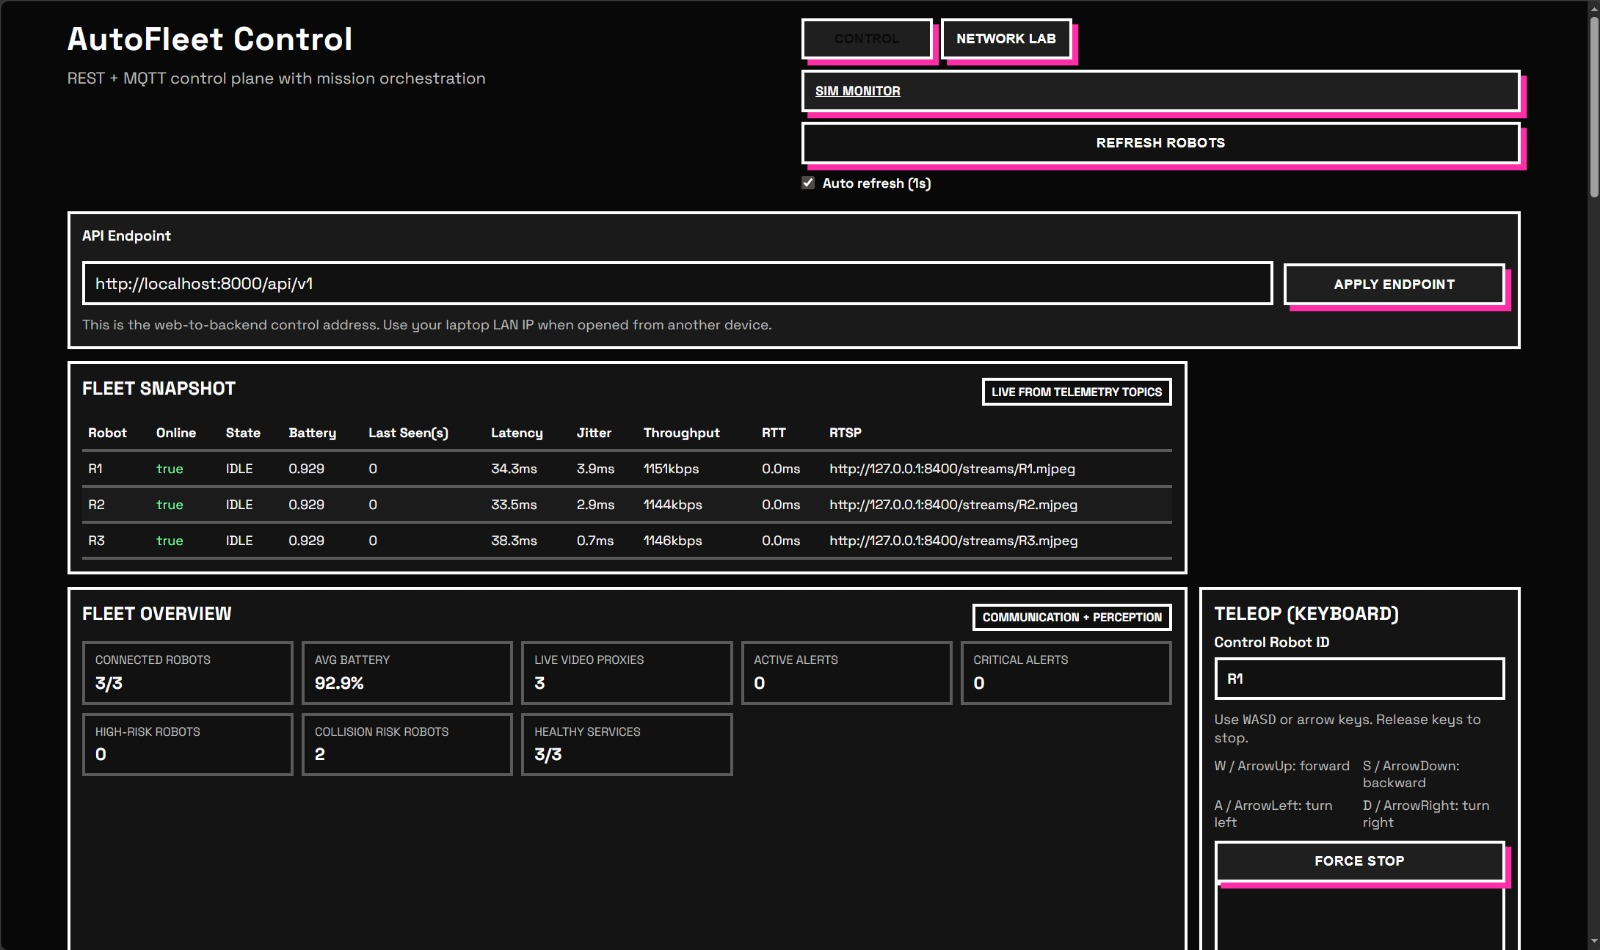
\includegraphics[width=0.92\textwidth]{images/7.jpg}
    \caption{Vue de diagnostic réseau et de gestion des flux vidéo}
    \label{fig:v2x_diagnostic_reseau}
\end{figure}

\section{Analyse des échanges et validation du système de supervision}

La validation de la supervision suppose une lecture conjointe des données effectivement échangées et des conditions réseau dans lesquelles ces échanges ont lieu.

\subsection{Données échangées et suivi de la flotte}

Les données manipulées dans Auto Fleet n’ont ni la même temporalité ni la même criticité. Les \kw{commandes} sont peu volumineuses mais sensibles. La \kw{télémétrie} est fréquente, régulière et utile à la lecture instantanée de l’état du système. Les \kw{événements} sont moins nombreux, mais souvent plus significatifs pour l’opérateur.

À cela s’ajoutent les \kw{états robots} et les données liées à la \kw{cartographie}. Cette diversité impose au backend de hiérarchiser implicitement la valeur fonctionnelle des messages, au lieu de traiter chaque donnée comme un flux interchangeable.

Le \kw{Tableau~\ref{tab:donnees_flotte}} synthétise cette diversité.

\begin{table}[H]
\centering
\small
\renewcommand{\arraystretch}{1.15}
\begin{tabular}{|p{3.1cm}|p{2.4cm}|p{3.8cm}|p{4.6cm}|}
\hline
\textbf{Donnée} & \textbf{Fréquence} & \textbf{Taille relative} & \textbf{Usage principal} \\
\hline
Commande & faible & faible & action opérateur \\
\hline
Télémétrie & régulière & faible à moyenne & suivi temps réel \\
\hline
Événement & ponctuelle & faible & journal et alertes \\
\hline
État robot & régulière & faible & disponibilité et santé système \\
\hline
Mise à jour carte & variable & moyenne à élevée & SLAM partagé \\
\hline
Référence vidéo & ponctuelle & faible & accès au flux visuel \\
\hline
\end{tabular}
\caption{Nature des données manipulées dans la supervision}
\label{tab:donnees_flotte}
\end{table}

\subsection{Mesures réseau et qualité de service}

La qualité de service ne se mesure pas uniquement à la présence ou à l’absence d’un message. Elle dépend aussi du délai d’acheminement, de sa variabilité et de la charge globale que le système demeure capable de supporter.

La \kw{latence} donne une première lecture de la réactivité. Le \kw{RTT} des commandes complète cette information en reflétant le temps réellement perçu par l’opérateur entre l’envoi d’un ordre et la réception d’un retour. Le \kw{jitter} renseigne, quant à lui, sur la régularité de cette expérience.

La \kw{perte de messages} doit être analysée selon le type de flux concerné. Une télémétrie ponctuellement lacunaire peut rester acceptable dans une supervision non critique ; une perte sur une commande structurante ou sur un acquittement ne l’est pas dans les mêmes termes.

Le \kw{débit disponible} et le \kw{RSSI} complètent cette lecture. Ils permettent d’interpréter une dégradation non plus seulement comme un symptôme, mais comme le résultat d’une saturation, d’un affaiblissement radio ou d’une coexistence excessive de flux concurrents.

\begin{figure}[H]
    \centering
    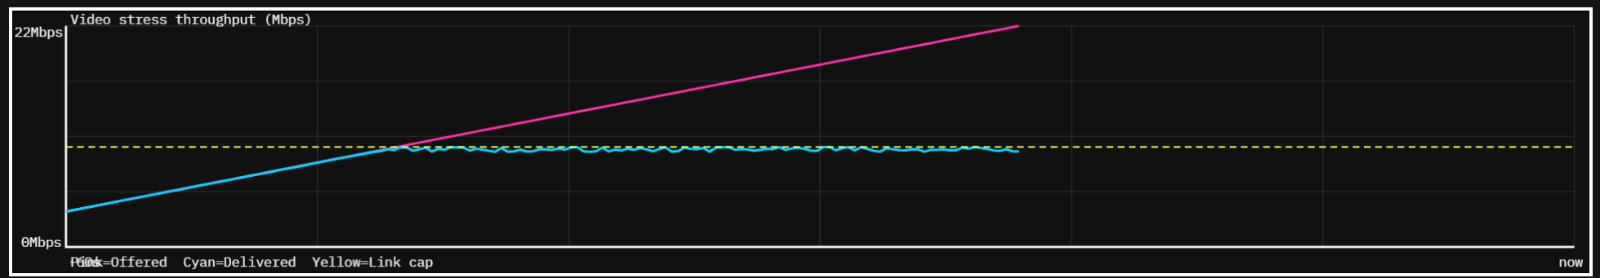
\includegraphics[width=0.92\textwidth]{images/8.jpg}
    \caption{Exemple de graphique de qualité de service réseau}
    \label{fig:v2x_qos_graph}
\end{figure}

\subsection{Limites observées et améliorations possibles}

La première limite de l’architecture actuelle tient à sa dépendance à la qualité effective du réseau. Même avec un découpage clair entre backend, broker et robots, la variabilité radio peut affecter la lisibilité de la supervision et la régularité des retours.

Une seconde limite concerne la \kw{densité informationnelle} de l’IHM. Une flotte multi-robots produit rapidement plus de données qu’il n’est raisonnable d’en afficher simultanément. L’interface doit donc hiérarchiser sans perdre l’essentiel, ce qui reste un problème d’ergonomie autant que de technique.

La vidéo constitue un troisième point de vigilance. Son intérêt est réel, mais son coût réseau est élevé. Une meilleure hiérarchisation des usages vidéo, voire une activation conditionnelle selon l’état du lien, améliorerait significativement la robustesse globale.

Enfin, la structuration des reconnexions, des accusés de réception et de la journalisation peut encore être renforcée. Une supervision plus robuste ne passe pas uniquement par de meilleurs graphes ou davantage d’écrans ; elle passe aussi par une causalité plus explicite entre l’événement observé et l’état réel du système.

% =========================
% CHAPITRE 6
% =========================
\fi

\chapter{Rendu final}

Ce chapitre est volontairement resserré. Il recevra, dans la version finale du manuscrit, la description stabilisée de ce qui est effectivement démontré : interface finale, scénarios retenus et résultats visibles du point de vue utilisateur.

\section{Interface utilisateur finale}

La description détaillée de l’IHM sera consolidée lorsque l’intégration complète des vues et des retours backend sera figée. Les rubriques suivantes sont conservées afin de structurer cette présentation finale.

\subsection{Organisation générale de l’IHM}

Cette sous-section documentera l’architecture visuelle finale de l’interface : répartition des panneaux, hiérarchie des blocs d’information, zones de commande, espace de retour mission et éventuelles vues cartographiques. L’objectif sera de justifier les choix d’organisation au regard de la \kw{charge cognitive} imposée à l’opérateur.

\subsection{Interactions entre l’utilisateur et le système}

Le texte final précisera les interactions réellement exposées : sélection d’un robot, émission d’ordres, changement de mode, lancement ou interruption de scénario, ainsi que les confirmations ou refus d’exécution remontés par le système. La distinction entre \kw{commande opérateur} et \kw{autonomie embarquée} devra y rester explicite.

\subsection{Informations affichées et retour du système}

Cette sous-section recensera les informations considérées comme essentielles à l’usage : état de connexion, batterie, télémétrie, retour mission, alertes, diagnostics réseau et disponibilité des flux complémentaires. Une approche purement descriptive sera évitée au profit d’une lecture fonctionnelle de l’affichage.

\section{Tests utilisateur et certification}

Cette section rassemblera les éléments de validation du prototype du point de vue de l’usage. Elle devra distinguer ce qui relève d’un comportement démontré, d’un comportement partiellement stabilisé ou d’un comportement encore expérimental.

\subsection{Scénarios de test retenus}

Les scénarios retenus pour l’évaluation finale préciseront les conditions de démonstration, les tâches confiées à l’opérateur et les fonctions effectivement mobilisées. Il s’agira de décrire des cas d’usage lisibles, et non une accumulation de manipulations élémentaires.

\subsection{Résultats observés du point de vue utilisateur}

Cette sous-section présentera les résultats visibles à l’échelle de l’interface : cohérence des états affichés, réactivité perçue des commandes, pertinence des retours et lisibilité générale de la supervision.

\subsection{Autres tests et limites actuelles}

Les autres campagnes de validation --- robustesse, stabilité ou contraintes réseau --- seront synthétisées ici de manière à relier l’expérience utilisateur aux limites techniques encore présentes dans le prototype.

% =========================
% CHAPITRE 7
% =========================
\chapter{Gestion de projet}

La gestion de projet a joué un rôle important dans le déroulement du projet \textbf{Auto Fleet}. Le projet ne se limitait pas à un développement logiciel classique : il combinait de la mécanique, de l'électronique, de la communication, de la supervision, de la perception et de l'intégration physique. Cette diversité a rendu impossible une organisation strictement linéaire. Nous avons donc adopté une méthode de travail itérative, proche d'une démarche agile, afin de pouvoir avancer malgré les imprévus matériels et les ajustements techniques.
 Nous avons réparti le travail autour de grands axes : la construction du robot, la partie vision et perception, la cartographie, l'IHM, ainsi que la communication entre les robots et entre les robots et l'interface de supervision. Cette organisation nous a permis de travailler en parallèle tout en gardant des points de synchronisation réguliers.

%------------------------------------------------
\section{Méthode de gestion}

La méthode de gestion retenue repose sur une logique \textbf{agile et itérative}. Dans le cadre du projet de synthèse, une méthode classique comme le cycle en cascade ou le cycle en V n'était pas adaptée, car plusieurs choix techniques dépendaient des essais réels, de la disponibilité du matériel et des problèmes rencontrés pendant l'intégration.

Nous avons donc avancé par versions successives. Chaque période de travail avait pour objectif de produire un résultat observable, même partiel : un robot capable de bouger, une première communication PC-robot, une simulation exploitable, une lecture de capteurs, une interface de supervision ou encore une démonstration intermédiaire. Cette approche a permis de corriger progressivement les problèmes au lieu d'attendre la fin du projet pour réaliser l'intégration complète.

Des réunions avec les tuteurs ont été réalisées environ toutes les deux semaines. Ces réunions servaient à présenter l'état d'avancement, identifier les blocages, valider les choix techniques et redéfinir les priorités lorsque cela était nécessaire.

\subsection{Cycle de vie agile utilisé}

Le cycle de vie suivi pendant le projet peut être résumé en plusieurs itérations courtes. Chaque itération commençait par un objectif technique, puis se poursuivait par une phase de développement, de test, de correction et de revue avec les tuteurs.

\begin{table}[H]
\centering
\small
\renewcommand{\arraystretch}{1.25}
\begin{tabular}{|p{3.8cm}|p{5.3cm}|p{5.3cm}|}
\hline
\textbf{Étape de l'itération} & \textbf{Objectif} & \textbf{Application dans le projet} \\
\hline

\textbf{Développement} &
Produire une première version exploitable. &
Développement du code, préparation des fichiers 3D, tests de montage, création de scripts ou configuration de la communication. \\
\hline
\textbf{Test intermédiaire} &
Vérifier si la solution fonctionne dans un cas simple. &
Tests sur simulation, essais de montage, vérification des déplacements, échanges réseau simples, affichage dans l'IHM. \\
\hline
\textbf{Correction} &
Modifier la solution en fonction des problèmes observés. &
Réimpression de supports moteurs, correction du code, modification de la structure du châssis, adaptation du planning. \\
\hline
\textbf{Revue} &
Présenter l'avancement et décider de la suite. &
Réunions avec les tuteurs, bilan des blocages et choix des priorités pour l'itération suivante. \\
\hline
\end{tabular}
\caption{Cycle de travail itératif utilisé pendant le projet}
\label{tab:cycle_iteratif}
\end{table}

Cette méthode a été particulièrement utile pour la partie mécanique. En effet, certains éléments n'étaient pas disponibles au moment prévu ou ne correspondaient pas exactement aux besoins. Au lieu d'arrêter le projet, nous avons déplacé l'effort vers les tâches qui pouvaient continuer : simulation, communication, IHM, préparation des scripts et conception 3D.

\subsection{Organisation générale des axes de travail}

Le projet a été structuré autour de plusieurs axes techniques. Ces axes n'étaient pas indépendants, mais ils permettaient de répartir les tâches et de faire avancer plusieurs parties en parallèle.

\begin{table}[H]
\centering
\small
\renewcommand{\arraystretch}{1.25}
\begin{tabular}{|p{4.1cm}|p{6.2cm}|p{4.4cm}|}
\hline
\textbf{Axe de travail} & \textbf{Objectif principal} & \textbf{Exemples de travaux réalisés} \\
\hline
\textbf{Construction du robot} &
Concevoir et assembler une base mobile exploitable. &
Châssis, supports moteurs, intégration des composants, impression 3D, câblage, tests physiques. \\
\hline
\textbf{Commande et déplacement} &
Permettre au robot de se déplacer correctement et de manière contrôlée. &
Mouvements simples, PID, trajectoires, odométrie, stabilisation des déplacements. \\
\hline
\textbf{Vision, perception et capteurs} &
Exploiter les capteurs pour détecter l'environnement proche. &
Lecture LiDAR, traitement d'obstacles simples, exploitation des données, tests de perception. \\
\hline
\textbf{Cartographie et coordination} &
Préparer la représentation de l'environnement et la coordination des robots. &
Carte, flotte simulée, évitement simple, coordination basique, tests d'intégration. \\
\hline
\textbf{IHM et communication} &
Permettre le contrôle, l'affichage et la supervision du système. &
Communication PC-robot, communication robot-IHM, V2X, heartbeat, timeouts, IHM de démonstration. \\
\hline
\textbf{Validation et démonstration} &
Préparer une version présentable et répétable du projet. &
Tests globaux, script de lancement, vidéo de secours, slides, documentation technique. \\
\hline
\end{tabular}
\caption{Structuration du projet Auto Fleet par axes de travail}
\label{tab:axes_travail}
\end{table}

Cette structuration a permis de limiter les blocages. Par exemple, lorsque le châssis ou les supports moteurs n'étaient pas encore totalement prêts, le développement de l'IHM, de la communication et de la simulation pouvait continuer. À l'inverse, lorsque le robot devenait disponible, les efforts étaient recentrés sur les tests physiques et l'intégration.

\subsection{Planning prévisionnel et planning réalisé}

Le planning du projet s'est étendu principalement de février à mai 2026. Le planning prévisionnel prévoyait une progression régulière : montage du robot, premiers déplacements, lecture des capteurs, communication, pré-intégration, stabilisation puis préparation de la démonstration finale. En pratique, le planning réalisé a dû être adapté à cause des retards et des problèmes liés au matériel, notamment sur le châssis et les supports moteurs.

\begin{table}[H]
\centering
\small
\renewcommand{\arraystretch}{1.20}
\begin{tabular}{|p{3.2cm}|p{4.5cm}|p{4.5cm}|p{3.2cm}|}
\hline
\textbf{Période} & \textbf{Prévision initiale} & \textbf{Réalisation effective} & \textbf{Écart constaté} \\
\hline
\textbf{20 février -- 6 mars} &
Montage de base, alimentation, drivers moteurs, premiers mouvements, communication PC-robot. &
Travail lancé, mais dépendant de la disponibilité réelle du matériel et des ajustements mécaniques. &
Début ralenti par les contraintes matérielles. \\
\hline
\textbf{7 mars -- 30 mars} &
Odométrie, lecture LiDAR, traitement de données, calibration, premiers tests capteurs. &
Avancement logiciel et tests partiels, avec certains essais physiques décalés en raison du montage incomplet. &
Validation réelle plus lente que prévu. \\
\hline
\textbf{31 mars -- 7 avril} &
Pré-intégration technique, flotte simulée, V2X v1, sécurité, affichage et démonstration intermédiaire. &
La simulation et les briques logicielles ont permis de présenter une version intermédiaire exploitable. &
Objectif maintenu grâce à la simulation. \\
\hline
\textbf{8 avril -- 5 mai} &
Stabilisation des mouvements, coordination, robustesse réseau et tests globaux. &
Recentrage sur la robustesse : heartbeat, timeouts, corrections PID, tests physiques et nettoyage logiciel. &
Priorités adaptées aux problèmes observés. \\
\hline
\textbf{6 mai -- 20 mai} &
Version stable, IHM de démonstration, script de lancement,&
Préparation d'une version plus répétable pour la démonstration, avec simplification du lancement. &
Objectif global respecté avec adaptation. \\
\hline
\textbf{21 mai -- 12 juin} &
Slides, documentation
&
Finalisation des supports, préparation de la soutenance et sauvegarde vidéo. &
Phase réalisée comme prévu. \\
\hline
\end{tabular}
\caption{Comparaison entre le planning prévisionnel et le planning réalisé}
\label{tab:planning_previsionnel_reel}
\end{table}

Le planning réel n'a donc pas été une simple exécution du planning initial. Il a évolué selon les contraintes rencontrées. Les tâches liées à la mécanique ont parfois pris plus de temps que prévu, tandis que les tâches logicielles ou de simulation ont été avancées pour éviter une période d'attente.

\subsection{Versions intermédiaires prévues et réalisées}

La consigne du projet demandait de présenter les versions intermédiaires prévues et réalisées. Dans notre cas, ces versions correspondaient aux jalons techniques que nous avons utilisés pour suivre l'avancement du projet.

\begin{table}[H]
\centering
\small
\renewcommand{\arraystretch}{1.20}
\begin{tabular}{|p{2.4cm}|p{3.4cm}|p{5.2cm}|p{4.2cm}|}
\hline
\textbf{Version} & \textbf{Période / jalon} & \textbf{Objectif prévu} & \textbf{Résultat réalisé} \\
\hline
\textbf{V0} &
Fin février 2026 &
Disposer d'une base de robot en cours de montage, avec premiers tests matériels. &
Version partielle, ralentie par les problèmes de châssis et de supports moteurs. \\
\hline
\textbf{V1} &
6 mars 2026 &
Présenter une démonstration minimale du robot lors du rendez-vous tuteurs. &
Démonstration limitée, avec certaines parties encore en cours de stabilisation. \\
\hline
\textbf{V2} &
Mars 2026 &
Avancer sur la communication PC-robot, les capteurs et les premiers traitements. &
Communication et développements logiciels poursuivis, avec des tests parfois réalisés hors robot complet. \\
\hline
\textbf{V3} &
7 avril 2026 &
Pré-soutenance technique : montrer une architecture fonctionnelle à environ 70\%. &
Version intermédiaire basée sur l'intégration partielle, la simulation et les premiers modules testables. \\
\hline
\textbf{V4} &
20 mai 2026 &
Obtenir une version stable et une démonstration répétable. &
Version recentrée sur les fonctions essentielles : mouvement, communication, IHM, sécurité et lancement simplifié. \\
\hline
\textbf{Version finale} &
31 mai 2026 &
Préparer le pack de présentation, les slides, la documentation et une vidéo de secours. &
Supports finalisés pour la soutenance, avec une vidéo backup en cas d'instabilité de la démonstration réelle. \\
\hline
\end{tabular}
\caption{Versions intermédiaires prévues et réalisées pendant le projet}
\label{tab:versions_intermediaires}
\end{table}

Cette logique de versions a permis de garder une progression mesurable. Même lorsque le système complet n'était pas encore prêt, chaque version intermédiaire apportait une brique exploitable pour la suite.

%------------------------------------------------
\section{Répartition des tâches et outils de gestion}

La répartition des tâches a été organisée autour des quatre membres du groupe : \textbf{Massyl}, \textbf{Jianke}, \textbf{Josué} et \textbf{Karim}. Chaque membre avait un axe principal, mais la répartition a évolué pendant le projet selon les problèmes rencontrés et les besoins d'intégration.

\subsection{Répartition initiale des tâches}

La répartition initiale avait pour but de couvrir les principales briques du projet. Elle est présentée dans le tableau~\ref{tab:repartition_taches}.

\begin{table}[H]
\centering
\small
\renewcommand{\arraystretch}{1.25}
\begin{tabular}{|p{3cm}|p{4.4cm}|p{7cm}|}
\hline
\textbf{Membre} & \textbf{Responsabilité principale} & \textbf{Travaux associés} \\
\hline
\textbf{Massyl} &
Communication, contrôle et IHM &
Communication PC-robot, panneau de contrôle, V2X, flotte simulée, durcissement réseau, heartbeat, timeouts, IHM de démonstration et script de lancement. \\
\hline
\textbf{Jianke} &
Perception, LiDAR et coordination &
Exploitation des données de tests, traitement LiDAR, détection d'obstacles simples, pré-intégration perception, coordination basique et nettoyage algorithmique. \\
\hline
\textbf{Josué} &
Montage, capteurs et tests physiques &
Montage, alimentation stable, drivers moteurs, encodeurs, odométrie basique, lecture LiDAR brute, mode sécurité, tests physiques globaux et documentation montage/câblage. \\
\hline
\textbf{Karim} &
Commande, simulation et trajectoires &
Mouvements simples du robot, PID, IMU, calibration, fusion capteurs, stabilisation finale, optimisation des trajectoires, simulation et schémas techniques. \\
\hline
\textbf{Tous les membres} &
Validation finale &
Intégration globale, tests de démonstration, correction des problèmes, préparation des slides, vidéo de secours et soutenance. \\
\hline
\end{tabular}
\caption{Répartition des tâches entre les membres du groupe}
\label{tab:repartition_taches}
\end{table}

Cette répartition n'était pas figée. Les parties étaient fortement liées : l'IHM dépendait des données de communication, la cartographie dépendait de la stabilité de l'odométrie, et les tests physiques dépendaient de la qualité du montage mécanique. Il était donc nécessaire de conserver une organisation flexible.

\subsection{Évolution de la répartition pendant le projet}

Au cours du projet, la répartition des tâches a évolué en fonction des blocages et des périodes critiques. Lorsque le robot réel n'était pas encore complètement disponible, nous avons déplacé une partie du travail vers les développements réalisables sans matériel complet : simulation, interface, communication et préparation des scripts.

Les principales évolutions ont été les suivantes :
\begin{itemize}
    \item les tâches mécaniques ont demandé plus d'itérations que prévu, notamment pour les supports moteurs ;
    \item les développements logiciels ont parfois été avancés en parallèle pour compenser les retards matériels ;
    \item les phases d'intégration ont nécessité une collaboration plus forte entre les membres ;
    \item les dernières semaines ont été consacrées collectivement à la stabilisation, à la démonstration, aux slides et à la vidéo de secours.
\end{itemize}

\begin{table}[H]
\centering
\small
\renewcommand{\arraystretch}{1.25}
\begin{tabular}{|p{4cm}|p{5.3cm}|p{5.3cm}|}
\hline
\textbf{Situation rencontrée} & \textbf{Effet sur l'organisation} & \textbf{Réaction adoptée} \\
\hline
\textbf{Matériel non disponible ou incomplet} &
Certaines tâches de test physique ne pouvaient pas être réalisées immédiatement. &
Avancement en simulation, préparation de l'IHM et développement de la communication. \\
\hline
\textbf{Supports moteurs à ajuster} &
Le montage du robot a demandé plusieurs essais avant d'être exploitable. &
Modification des modèles 3D, passage par Blender et Bambu Studio, puis nouvelles impressions. \\
\hline
\textbf{Pré-soutenance technique} &
Besoin de présenter une version intermédiaire cohérente. &
Regroupement des efforts sur les briques démontrables : simulation, communication, perception et sécurité. \\
\hline
\textbf{Démonstration finale} &
Nécessité d'avoir une version simple à lancer et plus fiable. &
Préparation d'un script de lancement, tests filmés et vidéo de secours. \\
\hline
\end{tabular}
\caption{Évolution de l'organisation pendant le projet}
\label{tab:evolution_repartition}
\end{table}

Cette évolution montre que nous avons conservé une logique agile : les responsabilités principales existaient, mais elles pouvaient être adaptées lorsque le projet l'exigeait.

\subsection{Outils de gestion et de collaboration}

Plusieurs outils ont été utilisés pour gérer le projet, partager les fichiers, coordonner les tâches et produire les éléments techniques nécessaires.

\begin{table}[H]
\centering
\small
\renewcommand{\arraystretch}{1.25}
\begin{tabular}{|p{3.4cm}|p{5.2cm}|p{5.4cm}|}
\hline
\textbf{Outil} & \textbf{Utilisation dans le projet} & \textbf{Apport} \\
\hline
\textbf{Discord} &
Communication quotidienne, échanges rapides, partage de captures, messages d'organisation et résolution de problèmes. &
Permet de garder un contact régulier entre les membres et de réagir rapidement aux blocages. \\
\hline
\textbf{GitHub} &
Stockage et versionnement du code, partage des scripts et suivi des modifications. &
Évite la perte de fichiers, facilite le travail collaboratif et permet de conserver un historique du projet. \\
\hline
\textbf{Planning Gantt} &
Suivi des tâches, des périodes de travail, des jalons et des responsabilités. &
Donne une vue globale de l'avancement et permet d'identifier les périodes critiques. \\
\hline
\textbf{Bambu Studio} &
Préparation des impressions 3D, découpage des modèles, réglages d'impression et génération des fichiers pour l'imprimante. &
Indispensable pour fabriquer et corriger les supports moteurs et certaines pièces du châssis. \\
\hline
\textbf{Blender} &
Modification, vérification ou adaptation de fichiers 3D avant impression. &
Permet d'ajuster les dimensions, l'encombrement et la forme des pièces mécaniques. \\
\hline
\textbf{Outils de simulation} &
Tests de comportement avant validation sur robot réel. &
Permettent de continuer le développement même lorsque le matériel est indisponible ou instable. \\
\hline
\textbf{Documents partagés} &
Centralisation des informations, figures, schémas, comptes rendus et supports de présentation. &
Facilite la préparation du rapport, des slides et de la soutenance. \\
\hline
\end{tabular}
\caption{Outils utilisés pour la gestion et la collaboration}
\label{tab:outils_gestion}
\end{table}

Ces outils ont été utilisés de manière complémentaire. Discord servait surtout à la coordination rapide. GitHub permettait de conserver les versions du code. Bambu Studio et Blender étaient essentiels pour la partie mécanique et impression 3D. Le planning Gantt servait à garder une vision d'ensemble du déroulement du projet.

%------------------------------------------------
\section{Changements rencontrés au cours du projet}

Pour la partie libre du chapitre, nous avons choisi le thème suivant : \textbf{l'agilité du projet face aux changements pendant le projet et les réactions de l'équipe}. Ce thème correspond bien à notre expérience, car plusieurs changements concrets ont eu lieu pendant le projet, principalement autour du matériel, du châssis et de l'intégration.

\subsection{Problèmes matériels rencontrés}

Les principaux changements sont venus de la partie matérielle. Certains éléments n'étaient pas disponibles au moment prévu, tandis que d'autres ne correspondaient pas exactement aux besoins du projet. Le problème le plus marquant concernait le châssis et les pièces nécessaires à l'intégration des moteurs.

\begin{table}[H]
\centering
\small
\renewcommand{\arraystretch}{1.25}
\begin{tabular}{|p{4cm}|p{5.3cm}|p{5.3cm}|}
\hline
\textbf{Problème rencontré} & \textbf{Conséquence} & \textbf{Impact sur le projet} \\
\hline
\textbf{Matériel non livré à temps} &
Certains tests physiques ne pouvaient pas être faits au moment prévu. &
Décalage des validations réelles et nécessité d'avancer sur d'autres modules. \\
\hline
\textbf{Matériel reçu non adapté} &
Certaines pièces ne correspondaient pas exactement aux contraintes du robot. &
Modification du montage et ajustement des choix techniques. \\
\hline
\textbf{Châssis plus complexe à intégrer que prévu} &
Difficultés pour placer correctement moteurs, batterie, cartes et câblage. &
Allongement de la phase de montage et besoin de revoir l'organisation interne du robot. \\
\hline
\textbf{Supports moteurs à refaire} &
Les premières versions n'étaient pas parfaitement adaptées aux dimensions réelles. &
Plusieurs versions ont été modélisées, préparées et imprimées avant d'obtenir une solution exploitable. \\
\hline
\textbf{Tests physiques dépendants du montage} &
Impossible de valider correctement certains modules tant que le robot n'était pas stable. &
Utilisation plus importante de la simulation et report de certaines validations. \\
\hline
\end{tabular}
\caption{Principaux changements et problèmes matériels rencontrés}
\label{tab:problemes_materiels}
\end{table}

Ces problèmes ont montré que la mécanique devait être considérée comme une partie centrale du projet. Un retard sur le châssis ou un support moteur mal adapté pouvait bloquer plusieurs autres parties : les déplacements, l'odométrie, les tests de capteurs et la démonstration.

\subsection{Itérations sur les pièces 3D}

L'impression 3D a joué un rôle important dans la résolution des problèmes mécaniques. Pour les supports moteurs, nous avons dû passer par plusieurs versions avant d'obtenir une pièce utilisable. Chaque version permettait de corriger un défaut observé lors du montage réel.

Le processus suivi était le suivant :
\begin{enumerate}
    \item vérification ou adaptation du modèle 3D ;
    \item modification des dimensions ou des points de fixation avec Blender lorsque cela était nécessaire ;
    \item préparation de l'impression dans Bambu Studio ;
    \item impression de la pièce ;
    \item test de montage sur le châssis ;
    \item correction du modèle en fonction du résultat obtenu.
\end{enumerate}

\begin{table}[H]
\centering
\small
\renewcommand{\arraystretch}{1.25}
\begin{tabular}{|p{3.5cm}|p{5.5cm}|p{5.5cm}|}
\hline
\textbf{Élément corrigé} & \textbf{Problème observé} & \textbf{Correction apportée} \\
\hline
\textbf{Dimensions du support} &
La taille ne correspondait pas parfaitement à l'espace disponible sur le châssis. &
Modification du modèle 3D et réimpression de la pièce. \\
\hline
\textbf{Points de fixation} &
Certains trous ou alignements ne correspondaient pas correctement au moteur ou au châssis. &
Ajustement des positions dans le modèle avant nouvelle impression. \\
\hline
\textbf{Résistance de la pièce} &
Certaines zones pouvaient être trop fines ou fragiles. &
Renforcement de la géométrie et adaptation des paramètres d'impression. \\
\hline
\textbf{Encombrement} &
La pièce pouvait gêner d'autres composants ou le câblage. &
Simplification de la forme et optimisation de l'espace occupé. \\
\hline
\end{tabular}
\caption{Corrections réalisées sur les pièces imprimées en 3D}
\label{tab:iterations_3d}
\end{table}

Même si ces itérations ont pris du temps, elles ont permis d'obtenir une solution plus adaptée au robot réel. Cette partie illustre bien la logique agile du projet : tester, corriger, réimprimer, puis tester de nouveau.

\subsection{Conséquences sur l'organisation}

Les changements rencontrés ont modifié l'ordre réel des tâches. Certaines validations ont été reportées, tandis que d'autres ont été avancées. Cela a évité que le projet reste bloqué sur une seule difficulté.

Les conséquences principales ont été les suivantes :
\begin{itemize}
    \item les tests physiques ont parfois été décalés ;
    \item les développements logiciels ont été poursuivis en parallèle ;
    \item la simulation a été utilisée plus tôt et plus souvent ;
    \item la préparation de l'IHM et des scripts a permis d'avancer sans attendre la stabilisation complète du robot ;
    \item les dernières semaines ont été davantage concentrées sur la robustesse et la répétabilité de la démonstration.
\end{itemize}

Cette adaptation a permis de conserver une progression globale malgré les imprévus. Le projet n'a donc pas suivi exactement le planning initial, mais il a gardé une cohérence grâce à la réorganisation régulière des priorités.

%------------------------------------------------
\section{Réactions de l'équipe et solutions apportées}

Face aux changements rencontrés, nous avons mis en place plusieurs solutions pour limiter les retards et continuer à produire des résultats. Ces solutions concernent à la fois l'organisation, la simulation, l'impression 3D, la communication et la préparation de la démonstration finale.

\subsection{Poursuite du travail en parallèle}

La première réaction a été de ne pas attendre que tous les problèmes matériels soient résolus pour continuer le projet. Lorsqu'une partie était bloquée, nous avancions sur une autre. Par exemple, pendant que les supports moteurs étaient en cours de correction, il était possible de travailler sur la communication, l'IHM, les scripts ou la simulation.

\begin{table}[H]
\centering
\small
\renewcommand{\arraystretch}{1.25}
\begin{tabular}{|p{4cm}|p{5.5cm}|p{5.2cm}|}
\hline
\textbf{Blocage} & \textbf{Travail poursuivi en parallèle} & \textbf{Intérêt} \\
\hline
\textbf{Châssis non stabilisé} &
Simulation, communication PC-robot, préparation de l'IHM. &
Éviter l'arrêt complet du projet. \\
\hline
\textbf{Supports moteurs à corriger} &
Modélisation 3D, scripts, tests logiciels et préparation des scénarios. &
Utiliser le temps d'attente pour avancer sur les parties indépendantes. \\
\hline
\textbf{Tests physiques non reproductibles} &
Vidéo de secours, script de lancement et simplification de la démonstration. &
Sécuriser la soutenance et réduire les risques le jour de la présentation. \\
\hline
\textbf{Intégration complexe} &
Tests par modules avant regroupement complet. &
Identifier plus facilement l'origine des erreurs. \\
\hline
\end{tabular}
\caption{Réactions mises en place face aux blocages}
\label{tab:reactions_blocages}
\end{table}

Cette organisation a permis de maintenir une progression continue. Elle correspond directement au fonctionnement agile attendu dans un projet de synthèse.

\subsection{Utilisation de la simulation}

La simulation a servi de solution intermédiaire lorsque le robot réel n'était pas encore prêt ou pas assez stable. Elle a permis de tester des comportements, de vérifier des échanges de données et de préparer les scénarios avant les essais physiques.

La simulation a été utile pour :
\begin{itemize}
    \item tester les premiers comportements de déplacement ;
    \item préparer la logique de flotte ;
    \item vérifier certaines données utilisées par l'IHM ;
    \item simuler des positions ou des états de robots ;
    \item préparer la démonstration avant d'avoir un système réel totalement stable.
\end{itemize}

Elle n'a pas remplacé les tests réels, mais elle a permis de réduire les risques. Lorsque les tests physiques devenaient possibles, nous pouvions repartir d'une logique déjà partiellement validée.

\subsection{Adaptations techniques apportées}

Plusieurs adaptations techniques ont été réalisées pendant le projet afin de répondre aux problèmes rencontrés.

\begin{table}[H]
\centering
\small
\renewcommand{\arraystretch}{1.25}
\begin{tabular}{|p{4.1cm}|p{5.3cm}|p{5.2cm}|}
\hline
\textbf{Adaptation} & \textbf{Objectif} & \textbf{Résultat obtenu} \\
\hline
\textbf{Modification des fichiers 3D} &
Adapter les pièces aux dimensions réelles du robot. &
Supports plus adaptés au châssis et aux moteurs. \\
\hline
\textbf{Utilisation de Bambu Studio} &
Préparer correctement les impressions 3D. &
Impressions plus propres et meilleure maîtrise des paramètres. \\
\hline
\textbf{Utilisation de Blender} &
Modifier ou vérifier les modèles 3D avant impression. &
Correction plus rapide des problèmes de forme ou de dimensions. \\
\hline
\textbf{Durcissement réseau} &
Rendre la communication plus fiable. &
Ajout de mécanismes comme heartbeat, timeouts et gestion automatique des nœuds. \\
\hline
\textbf{Script de lancement} &
Simplifier le démarrage de la démonstration. &
Réduction des manipulations manuelles et des risques d'erreur. \\
\hline
\textbf{Vidéo de secours} &
Prévoir une solution en cas de problème le jour de la soutenance. &
Sécurisation de la présentation finale. \\
\hline
\end{tabular}
\caption{Adaptations techniques réalisées pendant le projet}
\label{tab:adaptations_techniques}
\end{table}

Ces adaptations ont permis de transformer certains blocages en étapes de correction. Elles montrent que les difficultés rencontrées n'ont pas seulement retardé le projet : elles ont aussi conduit à améliorer certaines parties, notamment la robustesse de la démonstration et la qualité de l'intégration.

\subsection{Bilan de la gestion agile}

Au final, la gestion du projet s'est appuyée sur trois principes principaux : avancer par versions intermédiaires, travailler en parallèle et adapter régulièrement les priorités. Cette méthode était adaptée à la nature du projet, car Auto Fleet combinait plusieurs domaines techniques fortement dépendants les uns des autres.

Le bilan de cette organisation est positif. Même si le planning initial a été modifié par les imprévus matériels, nous avons conservé une progression régulière. Les réunions avec les tuteurs ont permis de garder un cadre de suivi, les outils collaboratifs ont facilité la coordination, et les solutions comme la simulation ou l'impression 3D ont permis de continuer à avancer malgré les blocages.

Cette expérience montre que l'agilité n'a pas seulement été une méthode théorique dans notre projet. Elle a été nécessaire pour réagir aux difficultés concrètes : matériel incomplet, pièces à refaire, intégration plus longue que prévu, besoin de versions intermédiaires et préparation d'une démonstration finale fiable.



% =========================
% CHAPITRE 8
% =========================
\chapter{Conclusion et perspectives}

\section{Conclusion du projet}

Cette section synthétisera les objectifs atteints, les résultats effectivement obtenus et les limites structurelles demeurant ouvertes au terme du projet. Elle devra distinguer clairement les éléments \kw{démontrés}, \kw{partiellement stabilisés} ou encore \kw{prospectifs}.

\section{Perspectives d'amélioration du projet}

Les perspectives porteront notamment sur l’amélioration de la perception, la robustesse du \kw{SLAM collaboratif}, la fiabilisation réseau, l’enrichissement de l’IHM et la montée en maturité de l’architecture embarquée.

% =========================
% BIBLIOGRAPHIE
% =========================
\begin{thebibliography}{99}

\bibitem{thrun2005}
S. Thrun, W. Burgard, D. Fox, \textit{Probabilistic Robotics}, MIT Press, 2005.

\bibitem{siciliano2016}
B. Siciliano, O. Khatib, \textit{Springer Handbook of Robotics}, 2\textsuperscript{e} édition, Springer, 2016.

\bibitem{mqtt2019}
OASIS, \textit{MQTT Version 5.0}, Standard, 2019.

\bibitem{ros2docs}
Open Robotics, \textit{ROS 2 Documentation}, documentation technique.

\bibitem{slamtoolbox}
S. Macenski et al., \textit{slam\_toolbox}, documentation et dépôt logiciel.

\end{thebibliography}

% =========================
% ANNEXES
% =========================
\appendix
\chapter{Annexes}

Cette partie regroupera les schémas détaillés, extraits de configuration, résultats complémentaires de tests et éléments de support non intégrés au corps principal du rapport.

\end{document}
